\chapter{Neural Networks}
\label{chap:nn}
%=============================================================================

Chapter~\ref{chap:logreg} closed with a remark that was left deliberately
unexplained: logistic regression is a neural network with no hidden layer.  Its
linear predictor $\bm{x}^{T}\bm{\theta}$ is a single artificial neuron, its
sigmoid is that neuron's activation function, and its cross entropy is the loss
used to train classification networks throughout deep learning.  This chapter
makes good on the remark by inserting layers between the input and the output,
so that the features fed to the final sigmoid are themselves \emph{learned}
rather than given.

That single change buys a great deal and costs a great deal.  What it buys is
universality: a network with one hidden layer can approximate any continuous
function to arbitrary accuracy, which none of the linear models of the previous
chapters can do.  What it costs is every guarantee we have relied on.  The cost
function is no longer convex, so Section~\ref{sec:convexity} no longer applies
and we can no longer say that the minimum we find is the minimum that exists.
There is no closed form, no analogue of the normal equations, and no
Karush-Kuhn-Tucker conditions to check the answer against.  We are left with
gradient descent and the chain rule.

Fortunately the chain rule is enough.  The central result of this chapter,
backpropagation, is nothing more than Eq.~(\ref{eq:1-chainrule}) applied
systematically to a composition of layers, arranged so that the gradient with
respect to \emph{all} the parameters is obtained for the price of about two
forward passes.  It is the reverse-mode automatic differentiation of
Section~\ref{sec:autodiff}, specialised to the layered structure of a network
and written out by hand.

%=============================================================================
%  PART ONE: FROM ONE NEURON TO MANY
%=============================================================================

\section{Artificial neurons}
\label{sec:perceptron}

\index{artificial neuron}\index{perceptron}
\index{bias!in a neuron}
An artificial neuron takes several inputs, forms a weighted sum, adds a bias
and passes the result through a non-linear function.  Writing the inputs as
$x_i$, the weights as $w_i$ and the bias as $b$,
\begin{equation}
  y = f\left(\sum_{i=1}^{n}w_ix_i+b\right) = f(z),
  \qquad z = \sum_{i=1}^{n}w_ix_i+b,
  \label{eq:8-neuron}
\end{equation}
where $f$ is the \emph{activation function} and $z$ the \emph{activation} or
pre-activation.  The bias is needed for the same reason the intercept was
needed in Section~\ref{sec:scalingintercept}: without it the neuron is
constrained to pass through the origin.  Figure~\ref{fig:8-neuron} is
Eq.~(\ref{eq:8-neuron}) drawn: the weighted sum on the left, the bias entering
as an input of its own, and the non-linearity on the right.

\begin{figure}[htbp]
\centering
\begin{tikzpicture}[>=Latex,
  inp/.style={circle,draw=black!65,fill=Blue3!12,minimum size=8.5mm,
              inner sep=0pt,font=\small},
  bia/.style={circle,draw=black!65,fill=Red3!12,minimum size=8.5mm,
              inner sep=0pt,font=\small},
  sm/.style={circle,draw=black!65,fill=black!5,minimum size=10mm,inner sep=0pt},
  ac/.style={rectangle,rounded corners=1pt,draw=black!65,fill=green!12,
             minimum height=10mm,minimum width=10mm,inner sep=1pt},
  wl/.style={font=\footnotesize,fill=white,inner sep=1pt}]
  \node[inp] (x1) at (0, 2.10) {$x_1$};
  \node[inp] (x2) at (0, 1.10) {$x_2$};
  \node      (xd) at (0, 0.30) {$\vdots$};
  \node[inp] (xn) at (0,-0.55) {$x_n$};
  \node[sm] (S) at (3.60,0.78) {$\sum$};
  \node[ac] (F) at (5.60,0.78) {$f$};
  \node[bia] (b) at (3.60,-1.35) {$b$};
  \draw[->,black!70] (x1) -- node[wl,pos=0.62]{$w_1$} (S);
  \draw[->,black!70] (x2) -- node[wl,pos=0.62]{$w_2$} (S);
  \draw[->,black!70] (xn) -- node[wl,pos=0.62]{$w_n$} (S);
  \draw[->,black!70] (b)  -- (S);
  \draw[->,black!70] (S) -- node[above,font=\footnotesize]{$z$} (F);
  \draw[->,black!70] (F) -- ++(2.0,0) node[right,font=\small] {$y=f(z)$};
  \node[font=\footnotesize,align=center] at (3.60,2.35)
       {$z=\displaystyle\sum_{i=1}^{n}w_ix_i+b$};
  \node[font=\footnotesize,black!60] at (0,-1.35) {inputs};
  \node[font=\footnotesize,black!60] at (5.60,-1.35) {activation};
\end{tikzpicture}
\caption{The artificial neuron of Eq.~(\ref{eq:8-neuron}).  The inputs $x_i$
are combined linearly with the weights $w_i$, the bias $b$ is added -- it is
drawn as a separate input because that is what it is, an input permanently
fixed at one -- and the resulting pre-activation $z$ is passed through the
non-linear activation function $f$ to give the output $y$.  Taking $f$ to be
the identity gives linear regression, the logistic function gives logistic
regression, and the step function gives Rosenblatt's perceptron.}
\label{fig:8-neuron}
\end{figure}

Equation~(\ref{eq:8-neuron}) is not new.  Taking $f$ to be the identity gives
the linear model of Chapter~\ref{chap:lreg}; taking $f=\sigma$, the logistic
function of Eq.~(\ref{eq:5-sigmoid}), gives logistic regression exactly; taking
$f$ to be the step function gives the \emph{perceptron}, historically the first
machine learning model, mentioned in Section~\ref{sec:classification} as the
hard classifier that the soft one improved upon.  A neuron is a familiar object
under a new name.

In a network of such neurons the inputs $x_i$ to one neuron are the
\emph{outputs} of the neurons in the preceding layer.  A network is
\emph{fully connected} when each neuron receives a weighted sum of the outputs
of \emph{all} neurons in the previous layer, and \emph{feed-forward} when the
connections carry information in one direction only, from input to output, with
no cycles.

%----------------------------------------------------------------------
\section{Why one layer is not enough: the XOR problem}
\label{sec:xor}

\index{XOR problem}
The clearest motivation for hidden layers is a problem that a single neuron
provably cannot solve.  Consider the classical logic gates, with two binary
inputs $x_1,x_2$ and a binary target:

\begin{table}[htbp]
\centering
\renewcommand{\arraystretch}{1.2}
\setlength{\tabcolsep}{10pt}
\begin{tabular}{cc|ccc}
\toprule
$x_1$ & $x_2$ & AND & OR & XOR\\
\midrule
0 & 0 & 0 & 0 & 0\\
0 & 1 & 0 & 1 & 1\\
1 & 0 & 0 & 1 & 1\\
1 & 1 & 1 & 1 & 0\\
\bottomrule
\end{tabular}
\caption{The AND, OR and XOR gates.  The first two are linearly separable in
the plane; the third is not.}
\label{tab:gates}
\end{table}

Let us first try linear regression, using the design matrix of
Eq.~(\ref{eq:1-designmatrix}) with a column of ones for the intercept.

\begin{Python}{}
import numpy as np

X = np.array([[1, 0, 0], [1, 0, 1], [1, 1, 0], [1, 1, 1]], dtype=np.float64)
Xinv = np.linalg.pinv(X.T @ X)

for name, y in [("XOR", [0, 1, 1, 0]), ("OR", [0, 1, 1, 1]), ("AND", [0, 0, 0, 1])]:
    y = np.array(y, dtype=np.float64)
    theta = Xinv @ X.T @ y                     # Eq. (3.olssolution)
    print(f"{name}: theta = {np.round(theta, 3)}, "
          f"prediction = {np.round(X @ theta, 3)}")
\end{Python}

The output is
\begin{Python}{}
XOR: theta = [ 0.5 -0.  -0. ], prediction = [0.5 0.5 0.5 0.5]
OR:  theta = [0.25 0.5  0.5 ], prediction = [0.25 0.75 0.75 1.25]
AND: theta = [-0.25 0.5  0.5 ], prediction = [-0.25 0.25 0.25 0.75]
\end{Python}

Look at the first line.  For the XOR gate the fitted slopes are \emph{exactly
zero} and the model predicts $0.5$ for every input: the least-squares fit has
found that the best linear function of $x_1$ and $x_2$ is the constant one.
This is not a numerical accident.  For XOR the two classes sit at opposite
corners of the unit square, and any straight line separating $\{(0,1),(1,0)\}$
from $\{(0,0),(1,1)\}$ would have to pass on both sides of the square at once.
The OR and AND gates, by contrast, \emph{are} linearly separable, and the fitted
values do at least order the outputs correctly.

Replacing the linear model by logistic regression does not help, since it
changes the link function but not the linearity of the boundary:

\begin{Python}{}
from sklearn.linear_model import LogisticRegression

for name, y in [("XOR", [0, 1, 1, 0]), ("OR", [0, 1, 1, 1]), ("AND", [0, 0, 0, 1])]:
    y = np.array(y)
    logreg = LogisticRegression().fit(X, y)
    print(f"{name}: accuracy {logreg.score(X, y):.2f}")
\end{Python}

\begin{Python}{}
XOR: accuracy 0.50
OR:  accuracy 0.75
AND: accuracy 0.75
\end{Python}

Fifty per cent on XOR is exactly chance.  The verdict is unambiguous and it is
the historical one: a single layer of neurons, however trained, computes a
linear decision boundary and there are elementary problems that no linear
boundary solves.  This observation stalled the field for the better part of two
decades.

Figure~\ref{fig:xor} shows why, and the picture is more convincing than any
amount of algebra.  For AND and for OR a single straight line separates the
classes, and a single neuron computes exactly such a line.  For XOR the two
classes occupy opposite corners of the square, and no line can be drawn with
both filled squares on one side and both circles on the other.  The failure is
geometric, and it is complete: it is not that training was insufficient or the
learning rate poorly chosen, but that the model class does not contain a
solution.

\begin{figure}[htbp]
\centering
\includegraphics[width=0.98\textwidth]{BookFigures/chapter08_neural_networks/xor_problem}
\caption{The three gates of Table~\ref{tab:gates} in the plane.  AND and OR are linearly separable and a single neuron suffices; XOR is not, and no straight line separates the two classes.}
\label{fig:xor}
\end{figure}


The remedy is a \emph{hidden} layer.  With two hidden units the network can
form two intermediate features -- in effect, something like ``$x_1$ or $x_2$''
and ``not both'' -- and the output neuron combines them linearly.  Using the
implementation we develop in Section~\ref{sec:nncode}, a network with two
inputs, two hidden nodes and two outputs learns all three gates perfectly:

\begin{Python}{}
X = np.array([[0, 0], [0, 1], [1, 0], [1, 1]], dtype=float)

for name, y in [("XOR", [0, 1, 1, 0]), ("OR", [0, 1, 1, 1]), ("AND", [0, 0, 0, 1])]:
    y = np.array(y)
    net = NeuralNetwork([2, 2, 2], "sigmoid", "classification",
                        gamma=1.0, epochs=4000, batch_size=4,
                        rng=np.random.default_rng(7)).fit(X, y)
    print(f"{name}: accuracy {np.mean(net.predict(X) == y):.2f}, "
          f"predictions {net.predict(X)}")
\end{Python}

\begin{Python}{}
XOR: accuracy 1.00, predictions [0 1 1 0]
OR:  accuracy 1.00, predictions [0 1 1 1]
AND: accuracy 1.00, predictions [0 0 0 1]
\end{Python}

Two hidden units and a non-linearity are the whole of the difference between
$0.50$ and $1.00$.

\begin{notebox}
\textbf{Machine learning connection.} It is worth being precise about what the
hidden layer supplies, because it is easy to say ``non-linearity'' and stop
there.  A network with a hidden layer but \emph{linear} activations computes
$\bm{W}^{2}(\bm{W}^{1}\bm{x}+\bm{b}^{1})+\bm{b}^{2}$, which is again an affine
function of $\bm{x}$ -- the product of two matrices is a matrix, and no depth
of linear layers escapes linearity.  It is the composition of the linear map
with a \emph{non-linear} $f$ that creates new features, and it is the reason
every activation function in Section~\ref{sec:activations} is non-linear.  Seen
from Chapter~\ref{chap:lreg}, a network performs the basis
expansion~(\ref{eq:3-basisexpansion}) with basis functions that are themselves
fitted rather than chosen in advance.
\end{notebox}

%----------------------------------------------------------------------
\section{Multilayer perceptrons and other architectures}
\label{sec:mlp}

\index{multilayer perceptron}
\index{feed-forward network}\index{fully connected layer}
A fully connected feed-forward network with an input layer, one or more hidden
layers and an output layer, whose neurons carry non-linear activation
functions, is called a \emph{multilayer perceptron} (MLP).  This is the
architecture we shall analyse in detail, and it is the one for which
backpropagation takes its simplest form.

Several other architectures appear later in this book, and it is useful to know
what distinguishes them.  \index{convolutional neural network}\index{recurrent neural network}\index{autoencoder}
\emph{Convolutional} networks replace full
connectivity by a small kernel slid across the input, so that each unit sees
only a local patch and the weights are shared across positions; this encodes
translation invariance and drastically reduces the parameter count, which is
why they dominate image processing.  \emph{Recurrent} networks feed the output
of a layer back into itself at the next time step, giving the network a memory
and making it suitable for sequences; the exploding-gradient problem of
Section~\ref{sec:vanishing} is particularly acute there.  \emph{Autoencoders}
place a narrow bottleneck between an encoder and a decoder and are trained to
reproduce their own input, which forces the bottleneck to learn a compressed
representation -- the non-linear counterpart of the principal component
analysis of Section~\ref{sec:pca}.

%----------------------------------------------------------------------
\section{The universal approximation theorem}
\label{sec:universal}

\index{universal approximation theorem}
Why should we expect a multilayer perceptron to be able to represent anything
useful?  The answer is a theorem, or rather a family of theorems refined over
some thirty years, and it is worth stating carefully because the loose version
in circulation claims both too much and too little.

\paragraph{Cybenko's theorem.}
\index{Cybenko's theorem}\index{sigmoidal function}
The first result is due to Cybenko in 1989~\cite{cybenko1989}.  Let $\sigma$ be
any continuous \emph{sigmoidal} function, meaning one with the limits
\begin{equation}
  \sigma(z) \longrightarrow
  \begin{cases}
    1 & z\rightarrow+\infty,\\
    0 & z\rightarrow-\infty,
  \end{cases}
  \label{eq:8-sigmoidal}
\end{equation}
and let $F(\bm{x})$ be a continuous function on the unit cube in $d$
dimensions, $\bm{x}\in[0,1]^{d}$.  Then for every $\epsilon>0$ there exists a
network with a single hidden layer,
$f(\bm{x};\bm{\Theta})$ with $\bm{\Theta}=(\bm{W},\bm{b})$, such that
\begin{equation}
  \left|F(\bm{x})-f(\bm{x};\bm{\Theta})\right| < \epsilon
  \qquad\text{for all }\bm{x}\in[0,1]^{d} .
  \label{eq:8-cybenko}
\end{equation}
In words: \emph{any continuous function on the unit cube in $d$ dimensions can
be approximated by a one-layer sigmoidal network to arbitrary accuracy.}

\paragraph{A familiar shape of argument.}
Readers who have met the Stone-Weierstrass theorem for polynomial
approximation, or the convergence criteria for Fourier series, will recognise
the structure: a family of simple functions is shown to be dense in the space
of continuous functions on a compact set.  Cybenko's proof proceeds by
functional analysis, showing that if the closure of the span of the network
functions were not everything, a non-zero signed measure would annihilate it,
and then deriving a contradiction from the sigmoidal property.  The result is
an existence statement of exactly the kind Stone-Weierstrass provides for
polynomials, and it should be regarded with the same mixture of reassurance and
scepticism.

\paragraph{Hornik's extension.}
\index{Hornik's theorem}
Hornik~\cite{hornik1991} generalised the result in two directions.  First, the
activation need only be non-constant and bounded, not specifically sigmoidal.
Second, and more useful in a statistical setting, the approximation can be
stated in mean square rather than uniformly.  If the inputs are distributed
with density $p(\bm{x})$ on a domain $D$ and the target has finite second
moment,
\begin{equation}
  \mathbb{E}\left[\left|F(\bm{x})\right|^{2}\right]
   = \int_{\bm{x}\in D}\left|F(\bm{x})\right|^{2}p(\bm{x})\,d\bm{x} < \infty,
  \label{eq:8-horniksecond}
\end{equation}
then for every $\epsilon>0$ there is a network with
\begin{equation}
  \mathbb{E}\left[\left|F(\bm{x})-f(\bm{x};\bm{\Theta})\right|^{2}\right]
   = \int_{\bm{x}\in D}
     \left|F(\bm{x})-f(\bm{x};\bm{\Theta})\right|^{2}p(\bm{x})\,d\bm{x}
   < \epsilon .
  \label{eq:8-hornikapprox}
\end{equation}
Equation~(\ref{eq:8-hornikapprox}) is the statement one actually wants, because
it is the expected squared error of Section~\ref{sec:biasvariance} rather than
a worst case over a cube the data may never visit.  Hornik's second point was
that universality is a property of the two-layer \emph{architecture} and not of
any special feature of sigmoids.

\paragraph{What the condition really is.}
The conditions usually quoted -- non-constant, bounded, monotonically
increasing and continuous -- are \emph{sufficient but not necessary}.  They
were convenient for the original proofs, which leaned on the boundedness.  The
\index{Leshno-Lin-Pinkus-Schocken theorem}
sharp characterisation is due to Leshno, Lin, Pinkus and
Schocken~\cite{leshno1993}: a feed-forward network with one hidden layer is a
universal approximator \emph{if and only if} the activation function is not a
polynomial on any interval.

This is a much better statement, and it explains a good deal.  It tells us at
once that ReLU qualifies, although it is unbounded and so fails Cybenko's
hypothesis; that every function in Section~\ref{sec:activations} qualifies; and
that the one activation which does \emph{not} work is the linear one, which is
a polynomial of degree one -- recovering, from the general theory, the
elementary observation of the notebox in Section~\ref{sec:xor} that a network
of linear layers collapses to a single linear map.

\paragraph{Which functions can be approximated.}
The theorems concern \emph{continuous} functions on a compact domain.  A
discontinuous $F$ cannot in general be approximated uniformly -- near a jump,
any continuous approximant must be wrong somewhere -- although in the mean
square sense of Eq.~(\ref{eq:8-hornikapprox}) a network may still do perfectly
well, failing only on a set of small measure.  Compactness matters too: nothing
is claimed about behaviour outside the region where the approximation was
constructed, which is the formal counterpart of the practical warning in
Section~\ref{sec:nnlimitations} that networks extrapolate unpredictably.

\paragraph{What the theorems do not say.}
Three qualifications are essential, and all three are routinely forgotten.

First, the conditions apply to the \emph{hidden} layer only.  The output nodes
are taken to be linear, so as not to restrict the range of the output values; a
sigmoid output could never represent a function taking the value $7$.

Second, and most importantly, \emph{none of the proofs gives any relation
between the approximation error $\epsilon$ and the number of hidden nodes},
nor any bound on the magnitudes of $\bm{W}$ and $\bm{b}$.  The required width
may grow exponentially with the input dimension.  This gap can be closed, and
Section~\ref{sec:universalwidth} closes it for the rectifier in one dimension
with an explicit construction and an explicit width.  Worse, the theorems are pure
existence results: they assert that suitable weights exist and say nothing
whatever about whether gradient descent, on a non-convex cost, will find them.
A guarantee of representability is not a guarantee of learnability, and the
distance between the two is where the practical difficulty of deep learning
lives.

Third, universality is not by itself remarkable.  Polynomials are universal on
a compact interval by Stone-Weierstrass, and so are Fourier series, splines and
radial basis functions; none of these is regarded as a breakthrough.  What
distinguishes networks is not \emph{that} they approximate but how economically
they do so in high dimensions, and in particular that adding \emph{depth}
rather than width is empirically far more efficient.  There are functions
representable by a deep network with a number of units polynomial in the depth
which provably require exponentially many units in a shallow one.  The
classical theorem, which concerns a single hidden layer, says nothing about
this -- so the result that justifies the field's name is precisely the one the
theorem does not cover.  Section~\ref{sec:universaldepth} gives a case where
the separation can be proved in half a page.

\begin{notebox}
\textbf{Machine learning connection.} A useful way to hold the theorem in mind
is to compare it with what we know about polynomials from
Chapter~\ref{chap:lreg}.  Polynomials are universal too, yet
Figure~\ref{fig:frankeselection} showed a degree-fourteen polynomial fit
failing catastrophically -- not because the function was unrepresentable but
because the coefficients could not be \emph{estimated} from a hundred noisy
points.  Universality is a statement about the model class; generalisation is a
statement about the model class, the data and the estimator together, and it is
governed by Eq.~(\ref{eq:2-biasvariance}) rather than by any approximation
theorem.  A network large enough to approximate anything is also large enough
to overfit anything, which is why Section~\ref{sec:nnregularisation} exists.
\end{notebox}

%......................................................................
\subsection{How wide?  A constructive bound}
\label{sec:universalwidth}

\index{universal approximation theorem!quantitative form}
The second qualification above -- that no proof relates $\epsilon$ to the
number of hidden nodes -- is a statement about \emph{those} proofs, not about
the problem itself.  For a rectified activation in one dimension the question
can be settled completely by an explicit construction, and it is worth doing,
because the construction is three lines long and answers exactly the question
the classical theorems evade.

The key observation is that a rectified network with one hidden layer is not
merely dense in the continuous functions: it \emph{is} the set of continuous
piecewise linear functions, and the number of pieces can be read off the width.

\begin{lemma}[Rectified networks are piecewise linear]
\label{lem:8-pieces}
Let
\begin{equation}
  g(x) = c + \sum_{i=1}^{N} v_i\,\mathrm{ReLU}\!\left(w_ix+b_i\right),
  \qquad x\in\mathbb{R},
  \label{eq:8-shallowrelu}
\end{equation}
be a network with one hidden layer of $N$ rectified units and a linear output.
Then $g$ is continuous and piecewise linear with at most $N+1$ affine pieces,
and every breakpoint lies in the set $\{-b_i/w_i : w_i\neq0\}$.
\end{lemma}

\begin{proof}
A unit with $w_i=0$ is constant and contributes no breakpoint.  A unit with
$w_i\neq0$ is affine on $(-\infty,-b_i/w_i]$ and affine on
$[-b_i/w_i,\infty)$, so the only point at which it fails to be affine is
$t_i=-b_i/w_i$.  The at most $N$ points $t_i$ cut the line into at most $N+1$
open intervals, and on each of them every summand of
Eq.~(\ref{eq:8-shallowrelu}) is affine; a finite sum of affine functions is
affine.  Continuity is inherited from the continuity of the rectifier.
\qed
\end{proof}

The converse is equally elementary -- any continuous piecewise linear function
with $N$ breakpoints can be written in the form~(\ref{eq:8-shallowrelu}) -- and
it is what makes the following bound constructive rather than existential.

\begin{theorem}[A width for every accuracy]
\label{thm:8-relurate}
Let $F$ be $L$-Lipschitz on $[a,b]$, that is $|F(x)-F(x')|\le L|x-x'|$ for all
$x,x'\in[a,b]$.  For every $N\ge1$ there is a network~(\ref{eq:8-shallowrelu})
with $N$ hidden rectified units such that
\begin{equation}
  \sup_{x\in[a,b]}\left|F(x)-g(x)\right| \;\le\; \frac{L(b-a)}{2N}.
  \label{eq:8-relurate}
\end{equation}
The hidden weights may all be taken equal to one and the hidden biases to
$-t_k$ with $t_k=a+k(b-a)/N$; only the $N+1$ output parameters depend on $F$.
\end{theorem}

\begin{proof}
Write $h=(b-a)/N$, $t_k=a+kh$ for $k=0,\dots,N$ and $y_k=F(t_k)$, and let
$s_k=(y_{k+1}-y_k)/h$ be the slope of the chord over $[t_k,t_{k+1}]$, with the
convention $s_{-1}=0$.  Define
\begin{equation}
  g(x) = y_0 + \sum_{k=0}^{N-1}\left(s_k-s_{k-1}\right)
              \mathrm{ReLU}\!\left(x-t_k\right).
  \label{eq:8-interpolant}
\end{equation}
For $x\in[t_m,t_{m+1}]$ every rectifier with $k\le m$ is active and every
rectifier with $k>m$ is not, so on that interval $g$ is affine with slope
$\sum_{k=0}^{m}(s_k-s_{k-1})=s_m$, the sum telescoping.  Since $g(t_0)=y_0$ and
the slope on $[t_k,t_{k+1}]$ is $s_k$, induction gives $g(t_k)=y_k$ for every
$k$: the network of Eq.~(\ref{eq:8-interpolant}) is exactly the piecewise
linear interpolant of $F$ at the $N+1$ knots.

It remains to bound the interpolation error.  Fix $x\in[t_m,t_{m+1}]$ and write
$x=t_m+\theta h$ with $\theta\in[0,1]$, so that
$g(x)=(1-\theta)y_m+\theta y_{m+1}$ and
\begin{equation}
  F(x)-g(x) = (1-\theta)\left(F(x)-F(t_m)\right)
            + \theta\left(F(x)-F(t_{m+1})\right).
  \label{eq:8-interperror}
\end{equation}
The Lipschitz property gives $|F(x)-F(t_m)|\le L\theta h$ and
$|F(x)-F(t_{m+1})|\le L(1-\theta)h$, whence
\begin{equation}
  \left|F(x)-g(x)\right| \le 2\theta(1-\theta)Lh \le \frac{Lh}{2},
  \label{eq:8-interpbound}
\end{equation}
the last step because $\theta(1-\theta)\le1/4$ on $[0,1]$.
\qed
\end{proof}

Equation~(\ref{eq:8-relurate}) is the missing relation.  Inverting it, accuracy
$\epsilon$ is reached with
\begin{equation}
  N = \left\lceil\frac{L(b-a)}{2\epsilon}\right\rceil
  \label{eq:8-widthforeps}
\end{equation}
hidden units -- an explicit, finite and entirely unmysterious width.  Nothing
in the proof is an existence argument: Eq.~(\ref{eq:8-interpolant}) writes the
weights down, and Fig.~\ref{fig:8-universal}(a) plots the resulting network for
$N=4$ and $N=16$.

\begin{notebox}
\textbf{The constant cannot be improved.}  Take
$F(x)=\mathrm{dist}(x,h\mathbb{Z})$, the triangular wave of period $h$, which is
$1$-Lipschitz.  It vanishes at every knot $t_k=kh$, so the interpolant of
Eq.~(\ref{eq:8-interpolant}) is identically zero, while $\sup|F|=h/2$.  The
bound~(\ref{eq:8-relurate}) is therefore attained exactly, and the factor two
in the denominator is the best possible for the class of $L$-Lipschitz
functions.
\end{notebox}

Both statements can be checked numerically.  The program \verb!universal.py!
builds the network of Eq.~(\ref{eq:8-interpolant}) -- it trains nothing -- and
measures its error on a grid of $200\,001$ points:

\begin{Python}{}
=== 1. the explicit construction of Theorem 8.relurate ===
  target F(x) = sin(2 pi x) on [0,1], Lipschitz constant L = 2 pi
     N    sup error   bound L/2N   ratio
     2    1.000e+00    1.571e+00   0.6366
     8    7.038e-02    3.927e-01   0.1792
    32    4.792e-03    9.817e-02   0.0488
   128    3.011e-04    2.454e-02   0.0123
   512    1.882e-05    6.136e-03   0.0031
\end{Python}

\begin{Python}{}
     N    sup error   bound L/2N   ratio
     2    2.500e-01    2.500e-01   1.0000
     8    6.250e-02    6.250e-02   1.0000
    32    1.562e-02    1.562e-02   1.0000
   128    3.905e-03    3.906e-03   0.9997
   512    9.763e-04    9.766e-04   0.9997
\end{Python}

The second table is the worst case of the notebox: the ratio is one to every
figure the grid can resolve, and the small shortfall at large $N$ is the
resolution of the grid, not a failure of the theory.  The first table says
something else worth noticing.  For a \emph{smooth} target the error falls like
$N^{-2}$, not like $N^{-1}$: that is the classical estimate
$\|F-g\|_\infty\le h^{2}\|F''\|_\infty/8$ for piecewise linear interpolation,
and it is the first sign that the Lipschitz class is a pessimistic yardstick.
Sharper rates of this kind, for deep rectified networks and for targets with
$s$ derivatives, are the subject of~\cite{yarotsky2017}; the whole
approximation-theoretic picture is surveyed in~\cite{pinkus1999}.

%......................................................................
\subsection{The curse of dimensionality}
\label{sec:universalcurse}

\index{curse of dimensionality}
Theorem~\ref{thm:8-relurate} is one-dimensional, and the dimension is where the
difficulty lies.  Repeating the construction on $[0,1]^{d}$ means covering the
cube with a grid of side $h$ and interpolating on it, which takes of the order
of $h^{-d}$ pieces; to reach accuracy $\epsilon$ for an $L$-Lipschitz target
one therefore needs of the order of
\begin{equation}
  N \;\sim\; \left(\frac{L\sqrt{d}}{2\epsilon}\right)^{d}
  \label{eq:8-curse}
\end{equation}
units.  With $L=1$ and $\epsilon=10^{-1}$ this is five units in one dimension,
about $10^{3}$ in three, and about $10^{12}$ in ten.  The exponent is the input
dimension, and no cleverness in the construction removes it.

Nor is this an artefact of the particular construction.  The class of
$L$-Lipschitz functions on $[0,1]^{d}$ contains, for every grid of side $h$, a
family of $2^{h^{-d}}$ functions obtained by placing a bump of height $Lh/2$ on
each cell with an independent sign; any two of them differ by $Lh/2$ somewhere,
so distinguishing them requires at least $h^{-d}$ bits and hence at least that
many parameters.  Made precise -- the parameters must be chosen by a map
depending continuously on the target -- this is the theorem of DeVore, Howard
and Micchelli~\cite{devore1989}: no approximation scheme with $N$ parameters
achieves error better than $c_dLN^{-1/d}$ uniformly over the Lipschitz ball.  A
network with one hidden layer of width $N$ has $N(d+2)+1$ parameters, so it is
covered by the theorem, and the exponent in Eq.~(\ref{eq:8-curse}) is sharp.

The way out is not a better architecture but a smaller class of targets.  The
classical result of this kind is Barron's~\cite{barron1993}.

\begin{theorem}[Barron]
\label{thm:8-barron}
Let $F:\mathbb{R}^{d}\rightarrow\mathbb{R}$ have a Fourier representation
$F(\bm{x})=\int e^{\imath\bm{\omega}\cdot\bm{x}}\hat{F}(\bm{\omega})\,d\bm{\omega}$
with finite first moment,
\begin{equation}
  C_F = \int \left\|\bm{\omega}\right\|
        \left|\hat{F}(\bm{\omega})\right| d\bm{\omega} < \infty .
  \label{eq:8-barronnorm}
\end{equation}
Then for every $N$ and every probability measure $\mu$ supported in the ball of
radius $r$ there is a network with one hidden layer of $N$ sigmoidal units for
which
\begin{equation}
  \int\left|F(\bm{x})-g(\bm{x})\right|^{2}\mu(d\bm{x})
   \;\le\; \frac{\left(2rC_F\right)^{2}}{N} .
  \label{eq:8-barron}
\end{equation}
\end{theorem}

The rate $N^{-1}$ in the squared error contains no $d$ at all.  The mechanism
deserves a sentence, because it explains where the dimension went.  The Fourier
representation exhibits $F-F(\bm{0})$ as a member of the closed convex hull of
a set $\mathcal{G}$ of individual ridge functions of norm at most $2rC_F$, so
$F$ is a limit of \emph{averages} of elements of $\mathcal{G}$; and if $N$
elements are drawn independently from the mixing distribution, the mean squared
error of their average is the variance of a single draw divided by $N$, which
is at most $(2rC_F)^{2}/N$.  Some particular draw must be at least as good as
the average, so a network of width $N$ with that error exists.  This averaging
argument is due to Maurey.  The dimension enters only through $C_F$, and for
the functions one actually wants to fit -- superpositions of a moderate number
of ridge directions, which is precisely what a network is -- $C_F$ does not
grow with $d$.

We can watch this happen.  The target
$F(\bm{x})=M^{-1}\sum_m c_m\cos(\kappa\,\bm{a}_m\cdot\bm{x})$ with $M=12$ unit
ridge directions has a Fourier transform consisting of point masses at
$\pm\kappa\bm{a}_m$, so its Barron norm is known exactly,
$C_F=\kappa M^{-1}\sum_m|c_m|$, and it does not depend on $d$; drawing $\bm{x}$
uniformly from the unit ball fixes $r=1$ in every dimension as well.
Theorem~\ref{thm:8-barron} therefore predicts the \emph{same} bound in
$d=1$, $5$ and $20$:

\begin{Python}{}
  kappa = 8:  C_F = 6.9124
      N       d = 1       d = 5      d = 20   bound (2 C_F)^2/N
      4   1.296e-02   2.689e-02   3.186e-02           4.778e+01
     16   2.330e-04   6.902e-03   2.202e-03           1.195e+01
     64   2.693e-04   1.247e-03   6.183e-04           2.986e+00
    128   1.850e-04   7.520e-04   6.779e-04           1.493e+00
  measured slopes of log(mse) against log(N):   -0.77  -1.08  -1.14   (Theorem 8.barron: -1)
  ratio of the d = 20 error to the d = 1 error at N = 128:  3.7
\end{Python}

Three things are worth reading off.  The bound holds, and with an enormous
margin -- it is a worst-case bound over the whole Barron class, and this
particular target is far from the worst.  The measured decay is close to the
predicted $N^{-1}$ in every dimension.  And the error at $d=20$ exceeds the
error at $d=1$ by a factor of under four, a constant, not by anything
resembling the exponential of Eq.~(\ref{eq:8-curse}).  It is the dimension in
the \emph{exponent} that the Barron class removes; a moderate constant remains.
Set against Eq.~(\ref{eq:8-curse}), where reaching a fixed accuracy at $d=20$
would take more units than there are atoms in the room, this is the whole
difference between a usable method and an impossible one.

%......................................................................
\subsection{Why depth?  An exact separation}
\label{sec:universaldepth}

\index{depth separation}
The third qualification -- that the classical theorem concerns one hidden layer
and so says nothing about depth -- can also be repaired, and in one dimension
the repair is completely elementary.  We exhibit a function that a deep network
of $2k$ units represents \emph{exactly}, and that no shallow network with fewer
than $2^{k}-1$ units can approximate at all.

\begin{definition}[The tent map and the sawtooth]
\label{def:8-tent}
Let
\begin{equation}
  T(x) = 2\,\mathrm{ReLU}(x) - 4\,\mathrm{ReLU}\!\left(x-\tfrac{1}{2}\right),
  \label{eq:8-tent}
\end{equation}
so that $T(x)=2x$ on $[0,\tfrac12]$ and $T(x)=2-2x$ on $[\tfrac12,1]$, and let
$s_k=T\circ T\circ\cdots\circ T$ be the $k$-fold composition.
\end{definition}

Equation~(\ref{eq:8-tent}) is one hidden layer of \emph{two} rectified units
followed by a linear combination.  Composing it $k$ times is therefore a
network with $k$ hidden layers of two units each: $2k$ units and $6k$
parameters in all.

\begin{lemma}[The sawtooth]
\label{lem:8-sawtooth}
$s_k$ maps $[0,1]$ onto $[0,1]$, is piecewise linear with exactly $2^{k}$
affine pieces of slope $\pm2^{k}$, and satisfies
\begin{equation}
  s_k\!\left(\frac{j}{2^{k}}\right)
   = \begin{cases} 0 & j \text{ even},\\ 1 & j \text{ odd},\end{cases}
  \qquad j = 0,1,\dots,2^{k}.
  \label{eq:8-sawvalues}
\end{equation}
\end{lemma}

\begin{proof}
Induction on $k$.  For $k=1$ the statement is Eq.~(\ref{eq:8-tent}).  Assume it
for $k$ and write $s_{k+1}=s_k\circ T$.  The map $T$ carries $[0,\tfrac12]$
affinely onto $[0,1]$ and carries $[\tfrac12,1]$ affinely onto $[0,1]$ with the
orientation reversed.  Hence $s_{k+1}$ restricted to $[0,\tfrac12]$ is a copy
of $s_k$ compressed by a factor two, and restricted to $[\tfrac12,1]$ is a
reflected copy: $2^{k}+2^{k}=2^{k+1}$ pieces in all, each of slope
$\pm2\cdot2^{k}$.  The points $j/2^{k+1}$ are the preimages of the points
$j/2^{k}$, and the alternation of the values is preserved by both branches.
\qed
\end{proof}

\begin{theorem}[Depth against width]
\label{thm:8-depth}
Let $g$ be a network with a single hidden layer of $N$ rectified units, as in
Eq.~(\ref{eq:8-shallowrelu}).  If $N\le2^{k}-2$ then
\begin{equation}
  \sup_{x\in[0,1]}\left|g(x)-s_k(x)\right| \;\ge\; \frac{1}{2}.
  \label{eq:8-depthsep}
\end{equation}
\end{theorem}

\begin{proof}
Suppose on the contrary that $\|g-s_k\|_\infty<\tfrac12$, and put
$x_j=j/2^{k}$ for $j=0,\dots,2^{k}$.  By Eq.~(\ref{eq:8-sawvalues}) we then
have $g(x_j)<\tfrac12$ for even $j$ and $g(x_j)>\tfrac12$ for odd $j$, so the
continuous function $g-\tfrac12$ changes sign on each of the $2^{k}$ intervals
$(x_j,x_{j+1})$ and has a zero $z_j$ in each.  These zeros are distinct and
ordered, $z_0<z_1<\cdots<z_{2^{k}-1}$.

No two consecutive zeros can lie in the same affine piece of $g$.  For if $z_j$
and $z_{j+1}$ both lay in a piece $P$, then $g-\tfrac12$ would be affine on $P$
with two distinct zeros and hence identically zero there; but
$x_{j+1}\in(z_j,z_{j+1})\subset P$, so $g(x_{j+1})=\tfrac12$, contradicting the
strict inequality above.  The $2^{k}$ zeros therefore lie in $2^{k}$ distinct
pieces, so $g$ has at least $2^{k}$ pieces, and Lemma~\ref{lem:8-pieces} gives
$N+1\ge2^{k}$.  This contradicts $N\le2^{k}-2$.
\qed
\end{proof}

The separation is exponential and it is exact.  A network of depth $k$ with two
units per layer -- $2k$ units, growing \emph{linearly} in $k$ -- reproduces
$s_k$ with no error whatever, while any network with a single hidden layer
needs at least $2^{k}-1$ units, growing \emph{exponentially}, merely to come
within a half.  At $k=10$ the deep network has twenty units and the shallow one
needs more than a thousand.

Both halves of the statement can be measured.  Composing the tent map and
counting the affine pieces of the result confirms Lemma~\ref{lem:8-sawtooth}:

\begin{Python}{}
     k   units in the deep net   linear pieces measured   2^k
     1                       2                        2      2
     4                       8                       16     16
     8                      16                      256    256
\end{Python}

Fitting shallow networks of increasing width to $s_3$, which has eight pieces
and therefore requires $N\ge7$, produces the wall the theorem predicts:

\begin{Python}{}
   k = 3, s_k has 8 pieces, the theorem needs N >= 7
      N   sup error   pieces of the fit   N+1
      2      0.5002                   2      3
      4      0.5212                   2      5
      8      0.5506                   6      9
     16      0.0096                  14     17
     32      0.0067                  25     33
     64      0.0031                  54     65
\end{Python}

The number of pieces never exceeds the $N+1$ of Lemma~\ref{lem:8-pieces}, and
whenever it falls below eight the error sits at or above the $1/2$ of
Theorem~\ref{thm:8-depth} -- including at $N=8$, where the width is sufficient
in principle but training produced a network with only six live pieces and the
theorem then applies to \emph{that} network.  The whole picture is
Fig.~\ref{fig:8-depth}.

Theorem~\ref{thm:8-depth} is the simplest member of a family.  Telgarsky proved
a version separating networks of any fixed depth from networks of slightly
smaller depth~\cite{telgarsky2016}, and Mont\'ufar and co-workers counted the
linear regions of a general rectified network~\cite{montufar2014}, finding a
number that grows exponentially in the depth but only polynomially in the
width.  The mechanism is always the one in Lemma~\ref{lem:8-sawtooth}:
composition \emph{multiplies} the number of pieces, addition merely adds them.
This is the result the name of the field refers to, and it is the one Cybenko's
statement cannot see.

\begin{figure}[htbp]
\centering
\includegraphics[width=0.98\textwidth]{BookFigures/chapter08_neural_networks/depth_separation}
\caption{Depth against width.  (a) The sawtooth $s_k$ of
Definition~\ref{def:8-tent}, computed exactly by a rectified network of depth
$k$ with two units per layer; the number of teeth doubles with each layer while
the number of units grows by two.  (b) Single-hidden-layer fits of $s_3$: at
$N=4$ and $N=8$ the network is flat at about $1/2$, which is the best a
function with too few pieces can do, and at $N=32$ it reproduces $s_3$ exactly.
(c) The measured supremum error against the width, with the threshold
$N=2^{k}-1$ of Theorem~\ref{thm:8-depth} marked by the dotted vertical lines
and the guaranteed error $1/2$ by the horizontal one.}
\label{fig:8-depth}
\end{figure}

%......................................................................
\subsection{Representability is not learnability}
\label{sec:universallearn}

\index{universal approximation theorem!and optimisation}
Every result so far is a statement about which functions a network
\emph{contains}.  Training is a different question, and the gap between the two
is not a technicality.  The construction of Theorem~\ref{thm:8-relurate} places
the kinks at $t_k=a+kh$ and computes the output weights directly from $F$;
gradient descent has to find both from a random start, on a cost function that
Section~\ref{sec:convexity} tells us is not convex.  Running the two side by
side at identical widths, on the same target $\sin2\pi x$:

\begin{Python}{}
     N   constructed   default init   kinks spread   ratio
     2     1.000e+00      1.000e+00      9.170e-01     0.9
     4     2.105e-01      1.108e+00      9.170e-01     4.4
     8     7.038e-02      1.837e-01      8.465e-02     1.2
    16     1.885e-02      7.203e-02      5.557e-02     2.9
    32     4.792e-03      4.279e-02      1.660e-02     3.5
    64     1.203e-03      4.386e-02      6.359e-03     5.3
\end{Python}

Two things are visible.  The first is that the default initialisation is a
handicap in its own right: PyTorch draws $w_i$ and $b_i$ from
$\mathcal{U}(-1,1)$, so the kink $-b_i/w_i$ falls inside the interval of
interest for only a minority of the units, and the rest are dead from the
start, contributing nothing and receiving no gradient.  Spreading the kinks
uniformly over $[0,1]$ -- which is exactly where
Eq.~(\ref{eq:8-interpolant}) puts them -- improves matters at every width, and
is a concrete instance of the general point of
Section~\ref{sec:initialisation}.

The second is that even with the kinks well placed, training does not reach the
constructed network, and the shortfall grows with the width: a factor $1.2$ at
$N=8$ and $5.3$ at $N=64$.  The exception at $N=4$, where every seed lands in
the same poor local minimum, is a reminder that these are non-convex problems
and that the failure need not be monotone.  The theorem guarantees that a set
of weights exists; it says nothing about whether the trajectory of Adam passes
anywhere near them.  This is the honest reading of the universal approximation
theorem.  It removes representability as an excuse and leaves optimisation and
generalisation as the two real problems, which are the subjects of
Chapter~\ref{chap:optim} and of Section~\ref{sec:nnregularisation}
respectively.  Figure~\ref{fig:8-universal} collects the three measurements.

\begin{figure}[htbp]
\centering
\includegraphics[width=0.98\textwidth]{BookFigures/chapter08_neural_networks/universal_construction}
\caption{The quantitative content of Section~\ref{sec:universal}.  (a) The
network of Eq.~(\ref{eq:8-interpolant}), whose weights are written down rather
than trained, for $N=4$ and $N=16$ hidden rectified units; the markers are the
knots $t_k$ at which it interpolates.  (b) Supremum error against width: the
bound~(\ref{eq:8-relurate}), the constructed network for a smooth and for a
worst-case Lipschitz target, and what Adam achieves at the same widths from two
initialisations.  The gap between the solid and the dashed curves is the
distance between representability and learnability.  (c) Barron's
rate~(\ref{eq:8-barron}) measured in $d=1$, $5$ and $20$ for two values of the
Barron norm; the slope is the predicted $-1$ and it does not change with the
dimension.}
\label{fig:8-universal}
\end{figure}

%=============================================================================
%  PART TWO: THE MATHEMATICS
%=============================================================================

\section{Notation and the feed-forward pass}
\label{sec:nnnotation}

\index{feed-forward pass}
We now fix notation, and it repays care: almost every difficulty students have
with backpropagation is a difficulty with indices rather than with calculus.

\index{layer!input}\index{layer!hidden}\index{layer!output}
Layers are numbered $l=0,1,\dots,L$, with $l=0$ the input layer, $l=L$ the
output layer, and $M_l$ the number of nodes in layer $l$.  The
\emph{activation} of node $j$ in layer $l$ is
\begin{equation}
  z_j^l = \sum_{i=1}^{M_{l-1}}w_{ij}^{l}a_i^{l-1}+b_j^{l},
  \label{eq:8-zdef}
\end{equation}
where $w_{ij}^{l}$ is the weight connecting node $i$ of layer $l-1$ to node $j$
of layer $l$, and $b_j^{l}$ is the bias of node $j$ in layer $l$.  The
\emph{output} of the node is obtained by applying the activation function,
\begin{equation}
  a_j^l = f\left(z_j^l\right),
  \label{eq:8-adef}
\end{equation}
with $a_i^{0}=x_i$ the network inputs.  In matrix-vector form,
Eqs.~(\ref{eq:8-zdef}) and (\ref{eq:8-adef}) become
\begin{equation}
  \boxed{\;
  \bm{z}^l = \left(\bm{W}^{l}\right)^{T}\bm{a}^{l-1}+\bm{b}^{l},
  \qquad
  \bm{a}^l = f\left(\bm{z}^l\right), \;}
  \label{eq:8-forward}
\end{equation}
with $f$ applied element-wise.  Evaluating Eq.~(\ref{eq:8-forward}) for
$l=1,\dots,L$ is the \emph{feed-forward pass}, and the network output is
$\tilde{\bm{y}}=\bm{a}^{L}$.

Figure~\ref{fig:8-mlp} shows the whole object with these labels attached, and
Figure~\ref{fig:8-node} shows a single node of it, which is where the index
convention has to be learned.  The point to fix in mind is that the superscript
on $w_{ij}^{l}$ names the layer the weight \emph{arrives} at, that the first
subscript names the node it \emph{leaves} and the second the node it arrives
at, and that the sum in Eq.~(\ref{eq:8-zdef}) is therefore over the first
index.  Every other convention in circulation is a permutation of this one, and
the only thing that matters is to choose one and never deviate from it.

\begin{figure}[htbp]
\centering
\begin{tikzpicture}[>=Latex,x=1cm,y=1cm,
  nd/.style={circle,draw=black!65,minimum size=9.5mm,inner sep=0pt,
             font=\footnotesize},
  inl/.style={nd,fill=Blue3!12},
  hd/.style={nd,fill=black!4},
  ou/.style={nd,fill=green!12},
  ed/.style={draw=black!25,-},
  hl/.style={draw=Red3,very thick,->}]
  \foreach \j/\y in {1/1.8,2/0.6,3/-0.6} \node[inl] (I\j) at (0,\y) {$a_{\j}^{0}$};
  \foreach \j/\y in {1/2.4,2/1.2,3/0,4/-1.2}
     \node[hd] (A\j) at (3,\y) {$a_{\j}^{1}$};
  \foreach \j/\y in {1/2.4,2/1.2,3/0,4/-1.2}
     \node[hd] (B\j) at (6,\y) {$a_{\j}^{2}$};
  \foreach \j/\y in {1/1.2,2/0} \node[ou] (O\j) at (9,\y) {$a_{\j}^{L}$};
  \foreach \i in {1,2,3} \foreach \j in {1,2,3,4} \draw[ed] (I\i) -- (A\j);
  \foreach \i in {1,2,3,4} \foreach \j in {1,2,3,4} \draw[ed] (A\i) -- (B\j);
  \foreach \i in {1,2,3,4} \foreach \j in {1,2} \draw[ed] (B\i) -- (O\j);
  \draw[hl] (A2) -- node[fill=white,inner sep=1pt,font=\footnotesize,pos=0.5]
        {$w_{23}^{2}$} (B3);
  \node[font=\footnotesize,align=center] at (0,-2.2)
       {input layer\\ $l=0$, $M_0=3$\\ $a_i^{0}=x_i$};
  \node[font=\footnotesize,align=center] at (3,-2.2)
       {hidden layer\\ $l=1$, $M_1=4$};
  \node[font=\footnotesize,align=center] at (6,-2.2)
       {hidden layer\\ $l=2$, $M_2=4$};
  \node[font=\footnotesize,align=center] at (9,-2.2)
       {output layer\\ $l=L$, $M_L=2$\\ $\tilde{\bm{y}}=\bm{a}^{L}$};
  \draw[->,black!55,thick] (0,3.5) --
       node[above,font=\footnotesize,black!55]
       {feed-forward pass, Eq.~(\ref{eq:8-forward})} (9,3.5);
\end{tikzpicture}
\caption{A fully connected feed-forward network in the notation of
Section~\ref{sec:nnnotation}, here with $L=3$.  Layer $l$ has $M_l$ nodes and
node $j$ of that layer carries the output $a_j^{l}$ of
Eq.~(\ref{eq:8-adef}); the input layer holds $a_i^{0}=x_i$ and the output
layer the prediction $\tilde{\bm{y}}=\bm{a}^{L}$.  Every node of one layer is
connected to every node of the next, and the highlighted edge carries the
weight $w_{23}^{2}$, from node $i=2$ of layer $l-1=1$ to node $j=3$ of layer
$l=2$: the superscript names the \emph{receiving} layer and the first index
names the \emph{sending} node.}
\label{fig:8-mlp}
\end{figure}

\begin{figure}[htbp]
\centering
\begin{tikzpicture}[>=Latex,x=1cm,y=1cm,
  nd/.style={circle,draw=black!65,minimum size=10mm,inner sep=0pt,
             font=\footnotesize},
  pr/.style={nd,fill=Blue3!12},
  nx/.style={nd,fill=green!12},
  bia/.style={circle,draw=black!65,fill=Red3!12,minimum size=8mm,
              inner sep=0pt,font=\footnotesize},
  wl/.style={font=\footnotesize,fill=white,inner sep=1pt}]
  \foreach \i/\y/\lab in {1/2.3/{a_{1}^{l-1}},2/1.1/{a_{2}^{l-1}},
                          4/-1.3/{a_{M_{l-1}}^{l-1}}}
     \node[pr] (P\i) at (0,\y) {$\lab$};
  \node at (0,0.0) {$\vdots$};
  \node[circle,draw=black!65,fill=orange!18,minimum size=19mm,inner sep=1pt,
        font=\footnotesize,align=center,text height=1.6ex,text depth=0.6ex]
        (J) at (4.2,0.5)
       {$z_j^{l}$\\$\big\downarrow$\\$a_j^{l}$};
  \node[bia] (b) at (4.2,-2.1) {$b_j^{l}$};
  \draw[->,black!70] (P1) -- node[wl,pos=0.58]{$w_{1j}^{l}$} (J);
  \draw[->,black!70] (P2) -- node[wl,pos=0.58]{$w_{2j}^{l}$} (J);
  \draw[->,black!70] (P4) -- node[wl,pos=0.58]{$w_{M_{l-1}j}^{l}$} (J);
  \draw[->,black!70] (b) -- (J);
  \foreach \k/\y/\lab in {1/1.7/{a_{1}^{l+1}},2/0.5/{a_{2}^{l+1}},
                          3/-0.7/{a_{3}^{l+1}}}
     \node[nx] (N\k) at (8.4,\y) {$\lab$};
  \foreach \k in {1,2,3}
     \draw[->,black!45] (J) -- node[wl,pos=0.55]{$w_{j\k}^{l+1}$} (N\k);
  \node[font=\footnotesize,align=center,anchor=north] at (4.2,-3.0)
       {$\displaystyle z_j^{l}=\sum_{i=1}^{M_{l-1}}w_{ij}^{l}a_i^{l-1}+b_j^{l},
         \qquad a_j^{l}=f\!\left(z_j^{l}\right)$};
\end{tikzpicture}
\caption{The index convention of Eqs.~(\ref{eq:8-zdef}) and (\ref{eq:8-adef}),
seen from a single node.  Node $j$ of layer $l$ collects the outputs
$a_i^{l-1}$ of all $M_{l-1}$ nodes of the previous layer, weighted by
$w_{ij}^{l}$, adds its own bias $b_j^{l}$ to form the pre-activation
$z_j^{l}$, and applies $f$ to obtain $a_j^{l}$, which it then sends on to every
node of layer $l+1$ through the weights $w_{jk}^{l+1}$.  The first index of a
weight always refers to the layer below and the second to the layer above, so
that the sum in Eq.~(\ref{eq:8-zdef}) runs over the first index and the sum in
the backpropagation equation~(\ref{eq:8-deltarecursion}) runs over the second.}
\label{fig:8-node}
\end{figure}

The cost of one forward pass is dominated by the matrix products: layer $l$
requires $M_{l-1}M_l$ multiplications, so the whole pass costs
$\bigO\!\left(\sum_l M_{l-1}M_l\right)$, which is also the number of weights.
This is why the operations of Chapter~\ref{chap:linalg} matter here: a network
is, computationally, a sequence of level-3 BLAS calls interleaved with
element-wise non-linearities, and Section~\ref{sec:arrays} explains why one
must let the library perform them.

\paragraph{Batches.}
\index{minibatch}
In practice one propagates a whole minibatch at once.  Stacking $n$ samples as
rows of $\bm{A}^{l-1}\in\mathbb{R}^{n\times M_{l-1}}$, the forward pass reads
\begin{equation}
  \bm{Z}^{l} = \bm{A}^{l-1}\bm{W}^{l}+\bm{b}^{l},
  \qquad
  \bm{A}^{l} = f\left(\bm{Z}^{l}\right),
  \label{eq:8-forwardbatch}
\end{equation}
with the bias added by broadcasting.  This is the form the code of
Section~\ref{sec:nncode} uses, and note that it transposes the convention of
Eq.~(\ref{eq:8-forward}): with samples in rows, $\bm{W}^{l}$ appears
untransposed.  Both conventions are common and mixing them is the single most
frequent source of shape errors.

%----------------------------------------------------------------------
\section{Activation functions}
\label{sec:activations}

\index{activation function}
The activation function must be non-linear, by the argument of the notebox in
Section~\ref{sec:xor} and by the sharp characterisation of
Section~\ref{sec:universal}, and for gradient-based training it must be
differentiable almost everywhere.  Beyond that the choice is open, and it
matters more than one might expect: the history of deep learning is to a
surprising extent the history of replacing one activation function by another.

The property to keep in view throughout is the \emph{derivative}, because it is
$f'$ and not $f$ that enters the backpropagation recursion~(\ref{eq:8-bp2}) and
therefore decides whether a gradient survives its passage through a layer.

%......................................................................
\subsection{Saturating activations}
\label{sec:satact}

The \emph{logistic} or sigmoid function of Eq.~(\ref{eq:5-sigmoid}),
\begin{equation}
  \sigma(z) = \frac{1}{1+e^{-z}},
  \qquad
  \sigma'(z) = \sigma(z)\left[1-\sigma(z)\right],
  \label{eq:8-sigmoid}
\end{equation}
was the standard choice for decades and is the one Cybenko's theorem was
proved for.  Its derivative is expressible in the function value alone, which
is convenient, and it never exceeds $\tfrac14$ -- which, as
Section~\ref{sec:vanishing} shows, is fatal in deep networks.  Its output is
also strictly positive with mean near $\tfrac12$, so the inputs to the next
layer are not centred, which slows learning further.

The \emph{hyperbolic tangent} $\tanh(z)=2\sigma(2z)-1$, with
$\tanh'(z)=1-\tanh^{2}(z)$, is a rescaled sigmoid mapping onto $(-1,1)$.  Its
output is centred on zero and its derivative reaches $1$ rather than
$\tfrac14$; it is consistently the better of the two and there is no good
reason to prefer the logistic function in a hidden layer.  Both nevertheless
saturate: for $|z|$ large the derivative is essentially zero and the unit stops
learning.

%......................................................................
\subsection{The rectified family}
\label{sec:reluact}

The \emph{rectified linear unit},
\begin{equation}
  \mathrm{ReLU}(z) = \max(0,z),
  \qquad
  \mathrm{ReLU}'(z) = \begin{cases}1 & z>0,\\ 0 & z<0,\end{cases}
  \label{eq:8-relu}
\end{equation}
broke the deadlock.  It is trivial to compute, it does not saturate for
positive arguments so the gradient passes through undiminished, and it produces
genuinely sparse activations since about half the units output zero.  Its
derivative is undefined at the origin, which in practice is assigned the value
zero and never noticed.

ReLU has one characteristic failure, the \emph{dying ReLU}.  If a unit's
weights are updated so that its input is negative for every training sample, it
outputs zero always; its gradient is then zero as well, so it can never
recover, and the unit is dead for the remainder of training.  With a large
learning rate a substantial fraction of a network can die this way -- in bad
cases half of it.

Three repairs give the negative branch a non-zero slope.  The \emph{leaky}
ReLU uses a fixed small slope,
\begin{equation}
  \mathrm{LReLU}(z) = \begin{cases} z & z>0,\\ \alpha z & z\le 0,\end{cases}
  \qquad \alpha\approx0.01,
  \label{eq:8-lrelu}
\end{equation}
so the gradient never vanishes entirely.  \emph{PReLU} makes $\alpha$ a
parameter learned by backpropagation like any other, one per channel.  The
\emph{exponential linear unit}
\begin{equation}
  \mathrm{ELU}(z) = \begin{cases}
    \alpha\left(e^{z}-1\right) & z<0,\\
    z & z\ge0,
  \end{cases}
  \label{eq:8-elu}
\end{equation}
does the same more smoothly, saturating at $-\alpha$ for large negative
arguments so that the unit output has a mean nearer zero, at the cost of an
exponential.  \emph{SELU} is ELU with two particular constants chosen so that,
under conditions on the initialisation, the activations of successive layers
converge to zero mean and unit variance automatically -- self-normalising, and
so an alternative to the batch normalisation of
Section~\ref{sec:nnregularisation}.

All of these are piecewise linear or piecewise smooth with a kink at the
origin.  The next family removes the kink.

%......................................................................
\subsection{Smooth gated activations: GELU and its relatives}
\label{sec:geluact}

\index{GELU}\index{Swish}\index{Mish}
The \emph{Gaussian error linear unit} takes a different view of what an
activation is doing.  Rather than thresholding the input, it \emph{weights the
input by the probability that it is positive}:
\begin{equation}
  \boxed{\;\mathrm{GELU}(z) = z\,\Phi(z),\;}
  \qquad
  \Phi(z) = \frac{1}{2}\left[1+\operatorname{erf}\!\left(\frac{z}{\sqrt{2}}\right)\right],
  \label{eq:8-gelu}
\end{equation}
where $\Phi$ is the cumulative distribution function of the standard normal
distribution met in Eq.~(\ref{eq:2-cdf}).  A unit whose input is large and
positive is passed through essentially unchanged, since $\Phi\to1$; one whose
input is large and negative is suppressed, since $\Phi\to0$; and in between the
suppression is graded rather than abrupt.  ReLU is the limiting case in which
$\Phi$ is replaced by the step function, that is in which the gating is
deterministic rather than probabilistic.

Because the error function is expensive, implementations use the
approximation
\begin{equation}
  \mathrm{GELU}(z) \approx \frac{z}{2}
    \left(1+\tanh\left[\sqrt{\frac{2}{\pi}}
      \left(z+0.044715\,z^{3}\right)\right]\right),
  \label{eq:8-geluapprox}
\end{equation}
which agrees with Eq.~(\ref{eq:8-gelu}) to better than $5\times10^{-4}$
everywhere on $[-8,8]$ and is what most frameworks compute by default.

Two close relatives replace the Gaussian gate by a cheaper one.  \emph{Swish},
also called \emph{SiLU}, gates with the logistic function,
\begin{equation}
  \mathrm{Swish}(z) = z\,\sigma(z),
  \label{eq:8-swish}
\end{equation}
and \emph{Mish} gates with a $\tanh$ of the softplus,
\begin{equation}
  \mathrm{Mish}(z) = z\tanh\left(\ln\left(1+e^{z}\right)\right).
  \label{eq:8-mish}
\end{equation}
The \emph{softplus} $\ln(1+e^{z})$ itself is a smooth approximation to ReLU and
appears mainly where a strictly positive output is needed, as when a network
predicts a variance.

\paragraph{What these functions have in common, and why it matters.}
All three are smooth, all three are \emph{non-monotone}, and all three have a
derivative exceeding one somewhere.  These are not incidental.

The non-monotonicity is easily quantified.  Each dips below zero for moderately
negative arguments before returning: GELU attains its minimum $-0.170$ at
$z=-0.752$, Swish $-0.278$ at $z=-1.279$, and Mish $-0.309$ at $z=-1.192$.  A
small negative response is therefore preserved rather than discarded, which is
the intended contrast with ReLU, and the function is not a squashing function
in the sense of any of the classical theorems -- it remains a universal
approximator because it is not a polynomial, by Section~\ref{sec:universal},
which is precisely the situation the sharper characterisation was needed for.

The derivative maxima are $1.129$ for GELU, $1.100$ for Swish and $1.089$ for
Mish, against $1$ for $\tanh$ and $\tfrac14$ for the sigmoid.  A factor
slightly greater than one in Eq.~(\ref{eq:8-deltaproduct}) means these
activations can mildly \emph{amplify} a gradient rather than only attenuate it,
which is a genuine advantage in depth; it also means they cannot be relied on
to damp an exploding gradient, so the clipping of
Section~\ref{sec:nnregularisation} remains necessary.

The smoothness matters for a reason that has nothing to do with
classification.  ReLU has a discontinuous first derivative and no second
derivative at the origin, so any method requiring curvature -- and any
application in which the network's \emph{output} is differentiated, as when
solving differential equations -- is compromised.  This is why the GELU family
is the default choice for physics-informed networks, a point we return to in
the next chapter.

\paragraph{Gated linear units.}
A final family generalises the idea by learning the gate.  A \emph{gated linear
unit} splits a layer's output in two and uses one half to gate the other,
\begin{equation}
  \mathrm{GLU}(\bm{z}) = \left(\bm{W}_1\bm{z}+\bm{b}_1\right)
    \circ \sigma\!\left(\bm{W}_2\bm{z}+\bm{b}_2\right),
  \label{eq:8-glu}
\end{equation}
with $\circ$ the Hadamard product.  Replacing the logistic gate by GELU gives
\emph{GeGLU} and by Swish gives \emph{SwiGLU}; the latter is used in most
current large language models.  Note that these are not activation
\emph{functions} in the sense of the rest of this section -- they are layers,
with their own parameters, and they double the number of weights for a given
output width.

%......................................................................
\subsection{Which activation should we use?}
\label{sec:whichact}

The empirical ordering, on which the literature is reasonably consistent, is
that the GELU and ELU families perform better than leaky ReLU and its variants,
which perform better than ReLU, which performs better than $\tanh$, which
performs better than the logistic function.

That ordering should be read with great caution, and it is worth measuring
rather than repeating.  Table~\ref{tab:actcompare} gives the test accuracy of a
network with three hidden layers of thirty units on the digits data, averaged
over five random seeds with the standard deviation across seeds.

\begin{table}[htbp]
\centering
\renewcommand{\arraystretch}{1.2}
\setlength{\tabcolsep}{12pt}
\begin{tabular}{lcc}
\toprule
\textbf{Activation} & \textbf{Test accuracy} & \textbf{Final training loss}\\
\midrule
sigmoid     & $0.8900\pm0.0096$ & $0.2971$\\
$\tanh$      & $\mathbf{0.9722\pm0.0039}$ & $0.0048$\\
ReLU        & $0.9672\pm0.0083$ & $0.0009$\\
leaky ReLU  & $0.9672\pm0.0071$ & $0.0009$\\
ELU         & $0.9672\pm0.0044$ & $0.0011$\\
GELU        & $0.9694\pm0.0061$ & $0.0010$\\
Swish       & $0.9661\pm0.0054$ & $0.0010$\\
Mish        & $0.9672\pm0.0048$ & $0.0010$\\
\bottomrule
\end{tabular}
\caption{Test accuracy of a $64$-$30$-$30$-$30$-$10$ network on the digits data
after $60$ epochs, as mean and standard deviation over five random seeds.  Only
the sigmoid is clearly separated from the rest.}
\label{tab:actcompare}
\end{table}

The table is worth more than the ordering it fails to confirm.  One result is
unambiguous: the sigmoid is far behind, by eight percentage points and many
standard deviations, and its training loss is two orders of magnitude higher --
with three hidden layers the attenuation of Section~\ref{sec:vanishing} is
already severe.  That much of the received wisdom is solidly reproduced.

The rest of the table is a single cluster.  The seven non-saturating
activations span $0.9661$ to $0.9722$, a range of $0.006$, while the standard
deviation across seeds is between $0.004$ and $0.008$ -- so \emph{the spread
between the methods is smaller than the spread between random seeds of the same
method}.  On this evidence the claimed ordering among them cannot be
distinguished from noise, and $\tanh$, which the ordering places second from
last, is nominally the best.  Note also that the training losses are nearly
identical while the test accuracies differ, so what little variation there is
comes from generalisation and not from optimisation.

The honest conclusion is that on a problem of this size the choice among the
non-saturating activations does not matter much, and that a paper reporting a
single run and declaring a winner among them would be reporting seed noise.
The differences do become real at greater depth, in transformers, and where the
smoothness itself is needed; they are not real here.  This is also a reminder
of Section~\ref{sec:clt}: with $360$ test samples the standard error of an
accuracy near $0.97$ is about $0.009$, so a difference of $0.006$ was never
going to be resolvable.  Figure~\ref{fig:actcompare} shows the same data
with error bars, which makes the point at a glance.

\begin{figure}[htbp]
\centering
\includegraphics[width=0.66\textwidth]{BookFigures/chapter08_neural_networks/activation_comparison}
\caption{The data of Table~\ref{tab:actcompare} plotted with error bars of one standard deviation over five seeds.  The shaded band spans the seven non-saturating activations; they are mutually indistinguishable, while the sigmoid lies far below.}
\label{fig:actcompare}
\end{figure}


Three further caveats apply to the literature ordering.  It is confounded with
architecture, since GELU rose to prominence together with transformers and is
best attested there.  Runtime matters: ReLU is a comparison and a multiplication, while GELU as computed by
Eq.~(\ref{eq:8-geluapprox}) requires a $\tanh$ and a cubic, which on large
models is not negligible.  If runtime is a concern, leaky ReLU with the default
$\alpha=0.01$ avoids both the dying-unit problem and the cost, without
introducing a hyperparameter worth tuning.

As a working rule: ReLU is a sound default and the right thing to try first;
move to leaky ReLU or ELU if units are dying; use GELU or Swish in transformers,
in very deep networks, and wherever the network output must be differentiated.
Reserve $\tanh$ for the cases where a bounded activation is genuinely wanted,
and use the logistic function in a hidden layer only when reproducing an old
result.

\begin{figure}[htbp]
\centering
\includegraphics[width=0.95\textwidth]{BookFigures/chapter08_neural_networks/gelu_detail}
\caption{Left: GELU, Swish and Mish against ReLU, with the minimum of each marked -- all three dip below zero and are therefore non-monotone.  Right: the error of the $\tanh$ approximation~(\ref{eq:8-geluapprox}) to the exact GELU~(\ref{eq:8-gelu}), which nowhere exceeds $4.7\times10^{-4}$.}
\label{fig:geludetail}
\end{figure}


Figure~\ref{fig:actfamilies} collects the three families with their
derivatives.  The bottom row is the one to study.  The saturating functions
have derivatives that vanish in both tails, and the sigmoid's never exceeds
$\tfrac14$; the rectified functions have derivative exactly one on the
positive axis and zero or nearly zero on the negative; the smooth gated
functions have derivatives that rise slightly \emph{above} one near the origin
and decay smoothly on both sides.  Reading the recursion~(\ref{eq:8-bp2})
through these three panels explains the empirical ordering better than any
list of benchmark numbers.

\begin{figure}[htbp]
\centering
\includegraphics[width=0.98\textwidth]{BookFigures/chapter08_neural_networks/activation_families}
\caption{Nine activation functions in three families (top) and their derivatives (bottom).  Only the derivative enters the backpropagation recursion~(\ref{eq:8-bp2}).  Dotted lines mark $\max\sigma'=1/4$ in the left panel and $f'=1$ in the other two.}
\label{fig:actfamilies}
\end{figure}


\paragraph{The output layer is not a free choice.}
Everything above concerns hidden layers.  The output activation is fixed by the
range of the target, exactly as the loss is fixed by its distribution in
Section~\ref{sec:maxlikelihood}: the identity for regression, the sigmoid for
binary classification, the softmax of Eq.~(\ref{eq:5-softmax}) for $K$ classes,
and softplus or an exponential where the output must be positive.  Choosing
these independently of the loss is one of the more common ways to produce a
network that trains to something meaningless.

%----------------------------------------------------------------------
\section{The cost function and the optimisation problem}
\label{sec:nncost}

\index{cost function!neural network}
Collect all weights and biases into a single parameter vector
$\bm{\Theta}=\{\bm{W}^{l},\bm{b}^{l}\}_{l=1}^{L}$.  Training means solving
\begin{equation}
  \hat{\bm{\Theta}} = \operatorname*{arg\,min}_{\bm{\Theta}}\;
    C\left(\bm{\Theta}\right),
  \qquad
  C(\bm{\Theta}) = \frac{1}{n}\sum_{i=1}^{n}
    L\left(y_i,\tilde{y}_i(\bm{\Theta})\right)
    + \lambda\,\Omega(\bm{\Theta}),
  \label{eq:8-cost}
\end{equation}
with $L$ the per-sample loss and $\Omega$ a regularisation term.  The loss is
chosen by the argument of Section~\ref{sec:maxlikelihood}: the half-squared
error for regression with Gaussian noise,
\begin{equation}
  C(\bm{\Theta}) = \frac{1}{2n}\sum_{i=1}^{n}
    \left(a_i^{L}-y_i\right)^{2},
  \label{eq:8-mse}
\end{equation}
and the cross entropy~(\ref{eq:5-crossentropy}) for classification, in its
multiclass form~(\ref{eq:5-multicrossentropy}) when $K>2$.

Three features distinguish Eq.~(\ref{eq:8-cost}) from every cost function so
far in this book.  It is \emph{not convex}: the composition of linear maps with
non-linearities destroys the property that Chapter~\ref{chap:optim} leaned on
so heavily, so there are many local minima and saddle points, and the minimum
we reach depends on the initialisation.  It is \emph{highly symmetric}:
permuting the units within a hidden layer, together with the corresponding
weights, leaves the function computed by the network unchanged, so every
minimum comes with a large family of equivalent copies.  And it has \emph{very
many parameters}, so the Hessian of Section~\ref{sec:newton} is out of the
question and we are restricted to the first-order methods of
Sections~\ref{sec:sgd} to \ref{sec:adam}.

That we nonetheless train such networks successfully is an empirical fact
rather than a theorem.  Part of the explanation is that in high dimensions
strict local minima are rare relative to saddle points, and that the many
symmetric copies of a good solution make some good solution easy to reach.

%----------------------------------------------------------------------
\section{Backpropagation}
\label{sec:backprop}

\index{backpropagation}
We now derive the gradient.  Everything follows from the chain
rule~(\ref{eq:1-chainrule}) and from two elementary derivatives of
Eq.~(\ref{eq:8-zdef}),
\begin{equation}
  \frac{\partial z_j^{l}}{\partial w_{ij}^{l}} = a_i^{l-1},
  \qquad
  \frac{\partial z_j^{l}}{\partial a_i^{l-1}} = w_{ij}^{l},
  \label{eq:8-zderivs}
\end{equation}
together with the derivative of the activation,
$\partial a_j^{l}/\partial z_j^{l}=f'(z_j^{l})$, which for the sigmoid is
$a_j^{l}(1-a_j^{l})$ by Eq.~(\ref{eq:8-sigmoid}).

\paragraph{The output layer.}
\index{error!of a node}\index{delta rule}
Take the squared-error cost~(\ref{eq:8-mse}) and specialise to $l=L$.
Differentiating with respect to a weight in the last layer,
\begin{equation}
  \frac{\partial C}{\partial w_{ij}^{L}}
   = \left(a_j^{L}-y_j\right)\frac{\partial a_j^{L}}{\partial w_{ij}^{L}}
   = \left(a_j^{L}-y_j\right)
     \frac{\partial a_j^{L}}{\partial z_j^{L}}
     \frac{\partial z_j^{L}}{\partial w_{ij}^{L}}
   = \left(a_j^{L}-y_j\right)f'\!\left(z_j^{L}\right)a_i^{L-1}.
  \label{eq:8-dCdwL}
\end{equation}
The structure of the result invites a definition.  Introduce the \emph{error}
of node $j$ in the output layer,
\begin{equation}
  \delta_j^{L}
   = f'\!\left(z_j^{L}\right)\frac{\partial C}{\partial a_j^{L}},
  \qquad\text{or in vector form}\qquad
  \bm{\delta}^{L} = f'\!\left(\bm{z}^{L}\right)\circ
    \frac{\partial C}{\partial \bm{a}^{L}},
  \label{eq:8-deltaL}
\end{equation}
where $\circ$ is the Hadamard product of Section~\ref{sec:vectors}.  With it,
Eq.~(\ref{eq:8-dCdwL}) becomes simply
\begin{equation}
  \frac{\partial C}{\partial w_{ij}^{L}} = \delta_j^{L}a_i^{L-1}.
  \label{eq:8-dCdwLcompact}
\end{equation}

Equation~(\ref{eq:8-deltaL}) is worth reading rather than merely recording.
The second factor measures how fast the cost changes with the $j$th output: if
the cost hardly depends on output $j$, then $\delta_j^{L}$ is small, which is
what one would want.  The first factor measures how fast the activation
function is changing at the value $z_j^{L}$ actually attained: a saturated unit,
with $f'\approx0$, contributes almost nothing however wrong it is.  That second
observation is the seed of the vanishing-gradient problem.

\paragraph{The error is the bias gradient.}
Note that $\delta_j^{L}$ can be written as
\begin{equation}
  \delta_j^{L} = \frac{\partial C}{\partial z_j^{L}}
   = \frac{\partial C}{\partial a_j^{L}}\frac{\partial a_j^{L}}{\partial z_j^{L}},
  \label{eq:8-deltaasdCdz}
\end{equation}
and since $\partial z_j^{L}/\partial b_j^{L}=1$ from Eq.~(\ref{eq:8-zdef}),
\begin{equation}
  \delta_j^{L} = \frac{\partial C}{\partial b_j^{L}} .
  \label{eq:8-deltaisbias}
\end{equation}
The error of a node \emph{is} the derivative of the cost with respect to that
node's bias.  This is not a coincidence but a consequence of the bias entering
$z$ additively, and it is why the same symbol serves both purposes.

\paragraph{Propagating the error backwards.}
It remains to obtain $\bm{\delta}^{l}$ for a general layer.  Define
$\delta_j^{l}=\partial C/\partial z_j^{l}$ as before, and express it through
the layer above.  Since $C$ depends on $z_j^{l}$ only through the activations
$z_k^{l+1}$ of the next layer, the chain rule gives
\begin{equation}
  \delta_j^{l}
   = \sum_k \frac{\partial C}{\partial z_k^{l+1}}
            \frac{\partial z_k^{l+1}}{\partial z_j^{l}}
   = \sum_k \delta_k^{l+1}\frac{\partial z_k^{l+1}}{\partial z_j^{l}} .
  \label{eq:8-deltachain}
\end{equation}
From $z_k^{l+1}=\sum_i w_{ik}^{l+1}a_i^{l}+b_k^{l+1}$ and
$a_i^{l}=f(z_i^{l})$ we obtain
$\partial z_k^{l+1}/\partial z_j^{l}=w_{jk}^{l+1}f'(z_j^{l})$, and therefore
\begin{equation}
  \boxed{\;
  \delta_j^{l} = \left(\sum_k \delta_k^{l+1}w_{jk}^{l+1}\right)
                 f'\!\left(z_j^{l}\right),
  \qquad
  \bm{\delta}^{l} = \left(\bm{W}^{l+1}\bm{\delta}^{l+1}\right)
                    \circ f'\!\left(\bm{z}^{l}\right). \;}
  \label{eq:8-deltarecursion}
\end{equation}
This is the backpropagation equation.  The error at a layer is the error at the
layer above, pulled back through the transpose of the weights and modulated by
the local derivative of the activation.  Figure~\ref{fig:8-backprop} draws it
next to the forward pass of Figure~\ref{fig:8-node}: the same graph, the same
weights, the arrows reversed.

\begin{figure}[htbp]
\centering
\begin{tikzpicture}[>=Latex,x=1cm,y=1cm,
  nd/.style={circle,draw=black!65,minimum size=10.5mm,inner sep=0pt,
             font=\footnotesize},
  lo/.style={nd,fill=orange!18},
  hi/.style={nd,fill=Blue3!12},
  wl/.style={font=\footnotesize,fill=white,inner sep=1pt}]
  \foreach \j/\y in {1/2.2,2/0.8,3/-0.6}
     \node[lo] (D\j) at (0,\y) {$\delta_{\j}^{l}$};
  \foreach \k/\y in {1/2.2,2/0.8,3/-0.6}
     \node[hi] (E\k) at (5.0,\y) {$\delta_{\k}^{l+1}$};
  \foreach \k in {1,2,3} \foreach \j in {1,2,3}
     \draw[<-,black!25] (D\j) -- (E\k);
  \foreach \k in {1,2,3}
     \draw[<-,Red3,thick] (D2) -- node[wl,pos=0.74]{$w_{2\k}^{l+1}$} (E\k);
  \node[font=\footnotesize,align=center,black!60] at (0,-1.9) {layer $l$};
  \node[font=\footnotesize,align=center,black!60] at (5.0,-1.9) {layer $l+1$};
  \draw[->,Red3,thick] (5.0,3.4) -- node[above,font=\footnotesize,Red3]
       {backward pass, Eq.~(\ref{eq:8-bp2})} (0,3.4);
  \node[font=\footnotesize,anchor=west] at (6.4,0.8)
       {$\displaystyle
         \delta_j^{l}=\left(\sum_k\delta_k^{l+1}w_{jk}^{l+1}\right)
         f'\!\left(z_j^{l}\right)$};
\end{tikzpicture}
\caption{The backward pass of Eq.~(\ref{eq:8-deltarecursion}), drawn on the
same network as Fig.~\ref{fig:8-node} but with the arrows reversed.  The error
$\delta_j^{l}$ of node $j$ in layer $l$ receives a contribution from
\emph{every} node $k$ of layer $l+1$, weighted by the same $w_{jk}^{l+1}$ that
carried $a_j^{l}$ forward, and the sum is then modulated by the local
derivative $f'(z_j^{l})$.  Comparing with Fig.~\ref{fig:8-node} shows what
backpropagation is: the identical graph traversed in the opposite direction,
with the transpose of each weight matrix in place of the matrix itself.  A
saturated node, one with $f'(z_j^{l})\approx0$, blocks the flow entirely, which
is the mechanism of Section~\ref{sec:vanishing}.}
\label{fig:8-backprop}
\end{figure}

%......................................................................
\subsection{The four equations of backpropagation}
\label{sec:backpropeqs}

Collecting the results gives the four equations on which everything rests:
\begin{align}
  \bm{\delta}^{L} &= f'\!\left(\bm{z}^{L}\right)\circ
    \frac{\partial C}{\partial\bm{a}^{L}},
  \label{eq:8-bp1}\\[4pt]
  \bm{\delta}^{l} &= \left(\bm{W}^{l+1}\bm{\delta}^{l+1}\right)
    \circ f'\!\left(\bm{z}^{l}\right),
  \label{eq:8-bp2}\\[4pt]
  \frac{\partial C}{\partial b_j^{l}} &= \delta_j^{l},
  \label{eq:8-bp3}\\[4pt]
  \frac{\partial C}{\partial w_{ij}^{l}} &= \delta_j^{l}a_i^{l-1}.
  \label{eq:8-bp4}
\end{align}
Equation~(\ref{eq:8-bp1}) starts the recursion at the output, (\ref{eq:8-bp2})
carries it backwards through the network, and (\ref{eq:8-bp3}) and
(\ref{eq:8-bp4}) convert the errors into the gradients we actually want.  Every
quantity on the right is already available: the $\bm{z}^{l}$ and $\bm{a}^{l}$
were computed during the forward pass and need only be stored, and $f'$ is a
cheap element-wise function.

\paragraph{A simplification worth knowing.}
For the two natural pairings of output activation and loss, the first equation
collapses.  With a linear output layer and the half-squared
error~(\ref{eq:8-mse}), $f'=1$ and $\partial C/\partial a_j^{L}=a_j^{L}-y_j$,
so
\begin{equation}
  \bm{\delta}^{L} = \bm{a}^{L}-\bm{y}.
  \label{eq:8-deltaLsimple}
\end{equation}
With a softmax output and the multiclass cross
entropy~(\ref{eq:5-multicrossentropy}), the derivative of the softmax and the
derivative of the logarithm cancel -- the same cancellation met in the notebox
of Section~\ref{sec:crossentropy} -- and Eq.~(\ref{eq:8-deltaLsimple}) holds
again.  In both cases the output error is simply prediction minus target, with
no factor of $f'$ to shrink it.  This is the deeper reason for pairing the
softmax with the cross entropy, and it is why the implementation of
Section~\ref{sec:nncode} treats both heads with one line of code.

\paragraph{Cost.}
\index{automatic differentiation!and backpropagation}
Counting operations, Eq.~(\ref{eq:8-bp2}) costs one matrix-vector product per
layer, exactly as the forward pass does.  The whole gradient with respect to
\emph{all} parameters therefore costs about twice a forward pass, independently
of the number of parameters.  This is precisely the claim made for reverse-mode
automatic differentiation in Section~\ref{sec:autodiff}, and backpropagation is
that algorithm specialised to a layered network.  Computing the same gradient
by finite differences, Eq.~(\ref{eq:4-gradcheck}), would require one forward
pass per parameter; for a network with $10^{6}$ weights the difference is
between a second and a fortnight.

%......................................................................
\subsection{The algorithm}
\label{sec:backpropalgo}

\index{training algorithm!feed-forward network}
Putting it together, training a feed-forward network proceeds as follows.

\paragraph{Set-up.}
\begin{enumerate}
  \item Fix the architecture: the number of inputs and outputs, the number of
        hidden layers and the number of nodes in each.
  \item Choose activation functions for the hidden layers and for the output
        layer, the latter dictated by the range of the target.
  \item Choose the cost function, again dictated by the distribution of the
        target, and any regularisation terms with their hyperparameters.
  \item Choose the optimiser from Chapter~\ref{chap:optim} -- plain gradient
        descent, momentum, RMSProp, Adam -- and its learning rate.
  \item Initialise the weights and biases, as discussed in
        Section~\ref{sec:initialisation}.
\end{enumerate}

\paragraph{Each iteration.}
\begin{enumerate}
  \item \emph{Forward pass.}  Set $\bm{a}^{0}=\bm{x}$ and compute
        $\bm{z}^{l}$ and $\bm{a}^{l}=f(\bm{z}^{l})$ for $l=1,2,\dots,L$ by
        Eq.~(\ref{eq:8-forward}), storing every $\bm{z}^{l}$ and $\bm{a}^{l}$.
  \item \emph{Output error.}  Compute $\bm{\delta}^{L}$ from
        Eq.~(\ref{eq:8-bp1}), or from Eq.~(\ref{eq:8-deltaLsimple}) for the
        natural pairings.
  \item \emph{Backward pass.}  For $l=L-1,L-2,\dots,1$ compute
        $\bm{\delta}^{l}$ from Eq.~(\ref{eq:8-bp2}).
  \item \emph{Gradients.}  Form
        $\partial C/\partial w_{ij}^{l}=\delta_j^{l}a_i^{l-1}$ and
        $\partial C/\partial b_j^{l}=\delta_j^{l}$.
  \item \emph{Update.}  With plain gradient descent and learning rate $\gamma$,
        \begin{equation}
          w_{ij}^{l}\leftarrow w_{ij}^{l}-\gamma\,\delta_j^{l}a_i^{l-1},
          \qquad
          b_j^{l}\leftarrow b_j^{l}-\gamma\,\delta_j^{l},
          \label{eq:8-update}
        \end{equation}
        or substitute any of the schemes of Chapter~\ref{chap:optim}.
\end{enumerate}
In practice steps 1--5 are applied to a minibatch rather than a single sample,
as in Section~\ref{sec:sgd}, and one pass over all minibatches is an epoch.

\begin{notebox}
\textbf{Machine learning connection.} \index{gradient checking}
Always verify a hand-written
backpropagation implementation against finite differences before trusting it.
Perturb one weight by $h\approx10^{-6}$, evaluate the cost twice, and compare
the central difference~(\ref{eq:4-gradcheck}) with the analytical gradient; the
relative discrepancy should be around $10^{-6}$ or smaller.  A wrong gradient
does not usually announce itself -- the network still trains, just to the wrong
place, or trains slightly worse than it should -- and this check takes minutes
to write.  The implementation of Section~\ref{sec:nncode} passes it at
$10^{-6}$ to $10^{-8}$ for every activation function and both output heads, and
those numbers are quoted there precisely so that a reader reimplementing it has
something to compare against.
\end{notebox}

%=============================================================================
%  PART THREE: MAKING IT WORK
%=============================================================================

\section{Vanishing and exploding gradients}
\label{sec:vanishing}

\index{vanishing gradients}\index{exploding gradients}
Backpropagation as derived above is correct, and for deep networks it does not
work.  Understanding why occupied the field for two decades and the explanation
is contained in Eq.~(\ref{eq:8-bp2}).

Unrolling the recursion from the output down to layer $l$,
\begin{equation}
  \bm{\delta}^{l} = \left[\prod_{k=l}^{L-1}
    \bm{W}^{k+1}\,\mathrm{diag}\left(f'(\bm{z}^{k})\right)\right]
    \bm{\delta}^{L},
  \label{eq:8-deltaproduct}
\end{equation}
so the gradient reaching layer $l$ is a product of $L-l$ factors.  A product of
many numbers each smaller than one shrinks geometrically; a product of many
numbers each larger than one grows geometrically.  Neither behaviour is
survivable.

In the first case the gradients reaching the early layers are so small that
gradient descent leaves those weights essentially unchanged, and training never
converges to a good solution.  This is the \emph{vanishing gradients} problem.
In the second the updates are so large that the iteration diverges: the
\emph{exploding gradients} problem, encountered particularly in recurrent
networks where the same weight matrix is applied at every time step.  More
generally, deep networks suffer from \emph{unstable} gradients, with different
layers learning at widely different speeds.

\paragraph{The sigmoid is the principal culprit.}
Consider the factors in Eq.~(\ref{eq:8-deltaproduct}) for the logistic
activation.  By Eq.~(\ref{eq:8-sigmoid}) the derivative $\sigma'$ never exceeds
$\tfrac14$, and it approaches zero rapidly once $|z|$ is large, so a saturated
unit contributes almost nothing.  Even in the best case, with every unit at its
most sensitive, ten layers multiply ten factors of at most $\tfrac14$, giving
$4^{-10}\approx10^{-6}$: the first layer receives a gradient a millionth of the
size of the last.  Sigmoid networks of any depth are, by construction, almost
untrainable at their input end.

Glorot and Bengio identified a second contribution in 2010.  With the then
standard initialisation -- weights drawn from $\mathcal{N}(0,1)$ -- the variance
of the outputs of each layer is considerably larger than the variance of its
inputs.  Going forward through the network the variance grows layer by layer
until the activations saturate at the top, and a saturated activation has a
vanishing derivative.  The logistic function makes matters worse still by
having mean $\tfrac12$ rather than zero, which is why $\tanh$, with mean zero,
behaves noticeably better in deep networks.

\paragraph{The two repairs.}
The first is the activation function.  ReLU does not saturate for positive
arguments and its derivative is exactly $1$ there, so the factors in
Eq.~(\ref{eq:8-deltaproduct}) do not shrink the gradient at all along the active
path.  This single change is most of the reason deep networks became trainable,
and the ReLU family of Section~\ref{sec:activations} is the standard choice for
that reason rather than for any biological one.

The second is initialisation, and it is the subject of the next section.

Figure~\ref{fig:vanishing} measures the effect directly.  For each network the
Frobenius norm of the weight gradient is plotted layer by layer after a single
backward pass.  With sigmoid activations the norm falls by orders of magnitude
from the output towards the input, and the deeper the network the more severe
the attenuation -- at eight hidden layers the first layer receives a gradient
several orders of magnitude smaller than the last, so it is effectively frozen.
With ReLU the profile is far flatter and the early layers continue to receive a
usable signal.  This is Eq.~(\ref{eq:8-deltaproduct}) made visible.

\begin{figure}[htbp]
\centering
\includegraphics[width=0.95\textwidth]{BookFigures/chapter08_neural_networks/vanishing_gradients}
\caption{Norm of the weight gradient at each layer after one backward pass, for networks of $1$, $2$, $4$ and $8$ hidden layers of $30$ units on the digits data.  Left: sigmoid activations, showing severe attenuation towards the input.  Right: ReLU, which preserves the gradient far better.}
\label{fig:vanishing}
\end{figure}


%----------------------------------------------------------------------
\section{Weight initialisation}
\label{sec:initialisation}

\index{weight initialisation}\index{Xavier initialisation}\index{He initialisation}
The argument of Glorot and Bengio is that for a signal to propagate properly we
need the variance of the outputs of each layer to equal the variance of its
inputs in the forward direction, and the variance of the gradients to be
preserved in the backward direction.

Suppose the inputs to a layer are independent with variance $\var(a)$, and the
$M_{l-1}$ weights are independent with mean zero and variance $\var(w)$.  Then
by the rules of Section~\ref{sec:expectation}, the activation
$z_j=\sum_i w_{ij}a_i$ has variance
\begin{equation}
  \var(z) = M_{l-1}\var(w)\var(a),
  \label{eq:8-varz}
\end{equation}
so $\var(z)=\var(a)$ requires $\var(w)=1/M_{l-1}$.  Repeating the argument for
the backward pass, where Eq.~(\ref{eq:8-bp2}) sums over the $M_l$ nodes of the
next layer, gives $\var(w)=1/M_l$.  The two conditions cannot both hold unless
the layers have equal width, and \emph{Xavier} or \emph{Glorot}
initialisation compromises between them,
\begin{equation}
  \var(w) = \frac{2}{M_{l-1}+M_l},
  \label{eq:8-xavier}
\end{equation}
drawing the weights from a Gaussian or a uniform distribution with this
variance.

For ReLU the argument needs one correction.  Since ReLU zeroes half of its
inputs on average, it halves the variance, and compensating for this gives
\emph{He} initialisation,
\begin{equation}
  \var(w) = \frac{2}{M_{l-1}},
  \label{eq:8-he}
\end{equation}
which is the appropriate choice for the whole ReLU family.  Biases are
initialised to zero, or to a small positive constant such as $0.01$ when using
ReLU, so that units start on the active side of the kink.

It is worth appreciating how much rests on Eq.~(\ref{eq:8-varz}).  Initialising
all weights to zero would make every unit in a layer compute the same thing and
receive the same gradient, so they would remain identical forever -- the
symmetry of Section~\ref{sec:nncost} must be broken by the initialisation.
Initialising them too large saturates the activations; too small and the signal
dies out. The permissible window is narrow, and Eqs.~(\ref{eq:8-xavier}) and
(\ref{eq:8-he}) locate it.

%----------------------------------------------------------------------
\section{Classification with neural networks}
\label{sec:nnclassification}

\index{softmax!in neural networks}
Classification requires only that the output layer and the loss be chosen
correctly, and both were determined in Chapter~\ref{chap:logreg}.

For $K$ classes the output layer has $K$ nodes and the softmax
activation~(\ref{eq:5-softmax}),
\begin{equation}
  a_k^{L} = \frac{\exp\left(z_k^{L}\right)}
                 {\sum_{l=0}^{K-1}\exp\left(z_l^{L}\right)},
  \label{eq:8-softmax}
\end{equation}
so that the outputs are non-negative and sum to one and may be read as class
probabilities.  As in Section~\ref{sec:softmax} the exponentials must be
computed after subtracting the largest score, Eq.~(\ref{eq:5-softmaxstable}),
or they overflow.  The loss is the multiclass cross
entropy~(\ref{eq:5-multicrossentropy}) with one-hot targets, and by the
cancellation noted after Eq.~(\ref{eq:8-deltaLsimple}) the output error is
simply $\bm{\delta}^{L}=\bm{a}^{L}-\bm{y}$.

The whole apparatus therefore reduces to multinomial logistic regression
applied to the \emph{learned} features $\bm{a}^{L-1}$ rather than to the raw
inputs.  A classification network is Chapter~\ref{chap:logreg} with a
representation learner bolted on in front, and this is the most useful way to
think about what the hidden layers are for.

%----------------------------------------------------------------------
\section{Regularisation and hyperparameters}
\label{sec:nnregularisation}

\index{regularisation!neural networks}\index{dropout}\index{batch normalisation}
A network with more parameters than data points can fit the training set
exactly, so the bias-variance considerations of
Section~\ref{sec:biasvariance} apply with full force and some form of control
is essential.

\paragraph{Weight penalties.}
Adding $\lambda\|\bm{\Theta}\|_2^{2}$ to Eq.~(\ref{eq:8-cost}) is the Ridge
penalty of Section~\ref{sec:ridge} under the name \emph{weight decay}; it
contributes $2\lambda\bm{W}^{l}$ to each weight gradient and nothing to the
bias gradients, since biases are not penalised for the reason given in
Section~\ref{sec:scalingintercept}.  An $\ell_1$ penalty produces sparse
weights exactly as in Section~\ref{sec:lasso}.

\paragraph{Early stopping.}
Monitor the cost on a validation set and stop when it begins to rise while the
training cost still falls.  This is the criterion of
Section~\ref{sec:schedules}, and for networks it is the single most effective
and cheapest regulariser available.

\paragraph{Dropout.}
During training, delete each unit independently with probability $p$, typically
$0.5$ for hidden layers, and rescale the survivors; at test time use the whole
network.  Each minibatch therefore trains a different thinned network, and the
final model behaves like an average over exponentially many of them -- which is
the variance reduction of Section~\ref{sec:whyensembles} obtained without
training an ensemble.  Dropout also prevents units from co-adapting, since no
unit can rely on any particular other unit being present.

\paragraph{Batch normalisation.}
Normalise the activations of a layer across the minibatch to zero mean and unit
variance, then rescale by two learned parameters.  This keeps the inputs of
each layer in the well-behaved region of its activation function and hence
attacks the vanishing-gradient problem directly; it also acts as a mild
regulariser, since the statistics depend on the composition of the minibatch.
The connection to Section~\ref{sec:learningrate} is exact: standardising the
inputs to a layer improves the conditioning of the optimisation problem that
layer poses, and Eq.~(\ref{eq:4-gdrate}) says what that is worth.

\paragraph{Gradient clipping.}
If the gradient norm exceeds a threshold, rescale it to that threshold.  This
does not cure exploding gradients but it prevents a single bad minibatch from
destroying the parameters, and it is standard practice in recurrent networks.

\paragraph{Hyperparameters.}
The number of hidden layers and their widths, the learning rate and its
schedule, the batch size, $\lambda$, the dropout rate and the activation
function are all hyperparameters, and they are chosen by the cross-validation
of Section~\ref{sec:crossvalidation} on a validation set -- never on the test
set.  Two rules of thumb survive contact with practice: the learning rate is by
far the most important, and it is usually better to build a network somewhat
too large and regularise it than to search for exactly the right size.

%=============================================================================
%  PART FOUR: IMPLEMENTATION
%=============================================================================

\section{A neural network from scratch}
\label{sec:nncode}

We now implement the whole of Sections~\ref{sec:nnnotation} to
\ref{sec:initialisation}.  The code follows the equations line for line, uses
the batched form~(\ref{eq:8-forwardbatch}) so that samples are rows throughout,
and handles both regression and classification.

\begin{Python}{}
import numpy as np


def sigmoid(z):
    """Numerically stable logistic function, Eq. (8.sigmoid)."""
    out = np.empty_like(z, dtype=float)
    p, n = z >= 0, z < 0
    out[p] = 1.0 / (1.0 + np.exp(-z[p]))
    e = np.exp(z[n]); out[n] = e / (1.0 + e)
    return out

def sigmoid_prime(z):  s = sigmoid(z); return s * (1 - s)
def relu(z):           return np.maximum(0.0, z)            # Eq. (8.relu)
def relu_prime(z):     return (z > 0).astype(float)
def leaky_relu(z, a=0.01):        return np.where(z > 0, z, a * z)
def leaky_relu_prime(z, a=0.01):  return np.where(z > 0, 1.0, a)
def elu(z, a=1.0):                                          # Eq. (8.elu)
    return np.where(z > 0, z, a * (np.exp(np.minimum(z, 0)) - 1))
def elu_prime(z, a=1.0):
    return np.where(z > 0, 1.0, a * np.exp(np.minimum(z, 0)))
def tanh_(z):          return np.tanh(z)
def tanh_prime(z):     return 1 - np.tanh(z)**2
def identity(z):       return z
def identity_prime(z): return np.ones_like(z)

def softplus(z):       return np.log1p(np.exp(-np.abs(z))) + np.maximum(z, 0)
def softplus_prime(z): return sigmoid(z)

def gelu(z):
    """Exact GELU, Eq. (8.gelu); erf comes from scipy."""
    from scipy.special import erf
    return z * 0.5 * (1.0 + erf(z / np.sqrt(2.0)))

def gelu_prime(z):
    from scipy.special import erf
    Phi = 0.5 * (1.0 + erf(z / np.sqrt(2.0)))
    phi = np.exp(-0.5 * z**2) / np.sqrt(2.0 * np.pi)      # the normal density
    return Phi + z * phi                                   # d/dz [z Phi(z)]

def gelu_tanh(z):
    """The approximation of Eq. (8.geluapprox) used by most frameworks."""
    return 0.5 * z * (1 + np.tanh(np.sqrt(2 / np.pi) * (z + 0.044715 * z**3)))

def swish(z):          return z * sigmoid(z)               # Eq. (8.swish)
def swish_prime(z):
    s = sigmoid(z); return s + z * s * (1 - s)

def mish(z):                                               # Eq. (8.mish)
    sp = np.log1p(np.exp(-np.abs(z))) + np.maximum(z, 0)
    return z * np.tanh(sp)

def mish_prime(z, h=1e-6):
    return (mish(z + h) - mish(z - h)) / (2 * h)           # numerical is adequate

def softmax(z):
    """Eq. (8.softmax), with the shift of Eq. (5.softmaxstable)."""
    e = np.exp(z - np.max(z, axis=1, keepdims=True))
    return e / np.sum(e, axis=1, keepdims=True)

ACT = {"sigmoid": (sigmoid, sigmoid_prime), "relu": (relu, relu_prime),
       "leaky_relu": (leaky_relu, leaky_relu_prime), "elu": (elu, elu_prime),
       "tanh": (tanh_, tanh_prime), "identity": (identity, identity_prime),
       "softplus": (softplus, softplus_prime), "gelu": (gelu, gelu_prime),
       "swish": (swish, swish_prime), "mish": (mish, mish_prime)}
\end{Python}

The network itself is short.  Note in particular \texttt{\_backward}, which is
Eqs.~(\ref{eq:8-bp1})--(\ref{eq:8-bp4}) transcribed.

\begin{Python}{}
class NeuralNetwork:
    """Fully connected feed-forward network trained by backpropagation.

    layer_sizes : e.g. [64, 50, 10] for 64 inputs, one hidden layer of 50
                  units and 10 outputs.
    task        : "classification" (softmax + cross entropy) or
                  "regression" (linear output + half-squared error).
    """

    def __init__(self, layer_sizes, hidden_activation="sigmoid",
                 task="classification", gamma=0.1, lmbd=0.0, epochs=100,
                 batch_size=32, rng=None):
        self.sizes, self.task = layer_sizes, task
        self.f, self.fp = ACT[hidden_activation]
        self.gamma, self.lmbd = gamma, lmbd
        self.epochs, self.batch = epochs, batch_size
        self.rng = np.random.default_rng(0) if rng is None else rng
        self._init_parameters(hidden_activation)

    def _init_parameters(self, act):
        """Xavier (8.xavier) or He (8.he) initialisation, by activation."""
        self.W, self.b = [], []
        for i in range(len(self.sizes) - 1):
            nin, nout = self.sizes[i], self.sizes[i + 1]
            s = np.sqrt(2.0 / nin) if act in ("relu", "leaky_relu", "elu") \
                else np.sqrt(1.0 / nin)
            self.W.append(self.rng.normal(0, s, (nin, nout)))
            self.b.append(np.zeros(nout) + 0.01)

    def _forward(self, X):
        """Eq. (8.forwardbatch); keeps every z and a for the backward pass."""
        a, z = [X], []
        for l in range(len(self.W)):
            zl = a[-1] @ self.W[l] + self.b[l]
            z.append(zl)
            if l == len(self.W) - 1:
                a.append(softmax(zl) if self.task == "classification" else zl)
            else:
                a.append(self.f(zl))
        return a, z

    def _backward(self, X, Y):
        """The four equations (8.bp1)-(8.bp4)."""
        n = X.shape[0]
        a, z = self._forward(X)

        # With softmax + cross entropy, and with a linear output under the
        # half-squared error, the output error is the same expression:
        delta = (a[-1] - Y) / n                       # Eq. (8.deltaLsimple)

        gW, gb = [None] * len(self.W), [None] * len(self.b)
        for l in range(len(self.W) - 1, -1, -1):
            gW[l] = a[l].T @ delta + self.lmbd * self.W[l]   # Eq. (8.bp4)
            gb[l] = np.sum(delta, axis=0)                    # Eq. (8.bp3)
            if l > 0:
                delta = (delta @ self.W[l].T) * self.fp(z[l - 1])  # Eq. (8.bp2)
        return gW, gb

    def fit(self, X, y):
        X = np.asarray(X, dtype=float)
        if self.task == "classification":
            self.classes_ = np.unique(y)
            idx = {c: i for i, c in enumerate(self.classes_)}
            Y = np.zeros((len(y), len(self.classes_)))        # one-hot
            Y[np.arange(len(y)), [idx[c] for c in y]] = 1
        else:
            Y = np.asarray(y, dtype=float).reshape(-1, 1)

        n = X.shape[0]
        self.loss_ = []
        for _ in range(self.epochs):
            order = self.rng.permutation(n)                   # shuffle, Sec. 4.practicaltips
            for s in range(0, n, self.batch):
                b = order[s:s + self.batch]
                gW, gb = self._backward(X[b], Y[b])
                for l in range(len(self.W)):                  # Eq. (8.update)
                    self.W[l] -= self.gamma * gW[l]
                    self.b[l] -= self.gamma * gb[l]
            self.loss_.append(self.cost(X, Y))
        return self

    def cost(self, X, Y):
        o = self._forward(X)[0][-1]
        if self.task == "classification":
            return float(-np.mean(np.sum(Y * np.log(np.clip(o, 1e-12, 1)), axis=1)))
        return float(0.5 * np.mean((o - Y)**2))               # Eq. (8.mse)

    def predict_proba(self, X):
        return self._forward(np.asarray(X, dtype=float))[0][-1]

    def predict(self, X):
        o = self.predict_proba(X)
        return (self.classes_[np.argmax(o, axis=1)]
                if self.task == "classification" else o.ravel())
\end{Python}

\paragraph{Verifying the gradient.}
Before using the network for anything we check \texttt{\_backward} against
finite differences, as urged in the notebox of
Section~\ref{sec:backpropalgo}.

\begin{Python}{}
def gradient_check(net, X, Y, h=1e-6, n_samples=15):
    """Compare backpropagation with the central difference (4.gradcheck)."""
    rng = np.random.default_rng(0)
    gW, gb = net._backward(X, Y)
    worst = 0.0
    for l in range(len(net.W)):
        for _ in range(n_samples):
            i = rng.integers(net.W[l].shape[0]); j = rng.integers(net.W[l].shape[1])
            net.W[l][i, j] += h; c1 = net.cost(X, Y)
            net.W[l][i, j] -= 2 * h; c2 = net.cost(X, Y)
            net.W[l][i, j] += h
            num = (c1 - c2) / (2 * h)
            worst = max(worst, abs(num - gW[l][i, j])
                        / (abs(num) + abs(gW[l][i, j]) + 1e-12))
    return worst
\end{Python}

Run over a three-hidden-layer network for every activation function, and over
regression as well as classification heads, the worst relative discrepancy is

\begin{Python}{}
classification, sigmoid                     1.38e-06
classification, tanh                        1.11e-08
classification, relu                        4.46e-07
classification, leaky_relu                  5.80e-07
classification, elu                         2.08e-08
classification, softplus                    1.48e-06
classification, gelu                        3.25e-07
classification, swish                       3.33e-08
classification, mish                        7.29e-08
regression, tanh                            3.55e-08
regression, relu, 2 hidden layers           1.19e-08
\end{Python}

which is the accuracy of the difference scheme itself.  The implementation of
Eqs.~(\ref{eq:8-bp1})--(\ref{eq:8-bp4}) is correct.

%----------------------------------------------------------------------
\section{Examples}
\label{sec:nnexamples}

\paragraph{Handwritten digits.}
The digits data set bundled with \texttt{scikit-learn} contains $1797$ images
of $8\times8$ pixels, giving $64$ inputs and $10$ classes.  We standardise the
features as urged in Section~\ref{sec:arrays}, hold out a fifth for testing,
and train a network with a single hidden layer of $50$ units.

\begin{Python}{}
import numpy as np
from sklearn.datasets import load_digits
from sklearn.model_selection import train_test_split
from sklearn.preprocessing import StandardScaler

digits = load_digits()
X = StandardScaler().fit_transform(digits.data)
X_train, X_test, y_train, y_test = train_test_split(X, digits.target,
                                                    test_size=0.2, random_state=42)

for activation in ["sigmoid", "relu"]:
    net = NeuralNetwork([64, 50, 10], activation, "classification",
                        gamma=0.1, lmbd=1e-4, epochs=60, batch_size=32,
                        rng=np.random.default_rng(2024)).fit(X_train, y_train)
    print(f"{activation:8s}: train {np.mean(net.predict(X_train) == y_train):.4f}  "
          f"test {np.mean(net.predict(X_test) == y_test):.4f}  "
          f"final loss {net.loss_[-1]:.4f}")
\end{Python}

\begin{Python}{}
sigmoid : train 0.9937  test 0.9722  final loss 0.0585
relu    : train 1.0000  test 0.9722  final loss 0.0059
\end{Python}

For comparison, \texttt{sklearn.neural\_network.MLPClassifier} with the same
architecture reaches $0.9778$ on the same split.  Our implementation is within
one test sample of a mature library, which is the appropriate standard.

The two activations reach the same test accuracy by different routes.  ReLU
drives the training loss an order of magnitude lower and fits the training set
exactly, while the sigmoid does not; that the test accuracies coincide means
the extra fitting bought nothing, which is the bias-variance story of
Section~\ref{sec:biasvariance} in a network.  With only one hidden layer the
vanishing-gradient argument of Section~\ref{sec:vanishing} has little room to
operate; its consequences appear when the depth grows, which is the subject of
one of the exercises.

Figure~\ref{fig:digits} shows the training curves and the effect of capacity.
On the left, ReLU drives the training cross entropy roughly an order of
magnitude below the sigmoid within sixty epochs, and $\tanh$ falls between
them -- the ordering the derivatives of Figure~\ref{fig:actfamilies} predict.
The test accuracies quoted in the legend are nevertheless within one sample of
one another, which is the reminder that a lower training loss is not the
objective.  On the right, accuracy against the number of hidden units shows the
familiar shape: rapid improvement up to about twenty units, then a plateau on
the test set while the training accuracy continues to unity.  The gap between
the two curves is the variance term of Eq.~(\ref{eq:2-biasvariance}).

\begin{figure}[htbp]
\centering
\includegraphics[width=0.95\textwidth]{BookFigures/chapter08_neural_networks/digits_training}
\caption{Left: training cross entropy against epoch for three hidden activations on the digits data, with the resulting test accuracies.  Right: training and test accuracy against the width of the single hidden layer.}
\label{fig:digits}
\end{figure}


\paragraph{Using established libraries.}
For anything beyond a teaching example one uses a framework, which supplies
automatic differentiation, GPU execution and a large catalogue of layers.  In
\texttt{scikit-learn},

\begin{Python}{}
from sklearn.neural_network import MLPClassifier

mlp = MLPClassifier(hidden_layer_sizes=(50,), activation="relu",
                    alpha=1e-4, max_iter=500, random_state=1)
mlp.fit(X_train, y_train)
print(f"test accuracy {mlp.score(X_test, y_test):.4f}")
\end{Python}

and in \texttt{PyTorch}, where the correspondence with our equations is
visible:

\begin{Python}{}
import torch
import torch.nn as nn

model = nn.Sequential(nn.Linear(64, 50),   # Eq. (8.forwardbatch)
                      nn.ReLU(),           # Eq. (8.relu)
                      nn.Linear(50, 10))   # softmax folded into the loss
loss_fn = nn.CrossEntropyLoss()            # Eq. (5.multicrossentropy)
optimiser = torch.optim.Adam(model.parameters(), lr=1e-3)   # Sec. 4.adam

Xt = torch.tensor(X_train, dtype=torch.float32)
yt = torch.tensor(y_train, dtype=torch.long)
for epoch in range(100):
    optimiser.zero_grad()
    loss = loss_fn(model(Xt), yt)
    loss.backward()                        # this is Eqs. (8.bp1)-(8.bp4)
    optimiser.step()                       # this is Eq. (8.update)
\end{Python}

The single call \texttt{loss.backward()} performs exactly the computation we
derived by hand, obtained by reverse-mode automatic differentiation over the
graph the forward pass recorded.  Knowing what it does is the point of having
derived it.

%----------------------------------------------------------------------
\section{Limitations, and a top-down view}
\label{sec:nnlimitations}

It is worth closing the exposition with some perspective, because the
enthusiasm surrounding neural networks makes it easy to lose.

Deep networks are extraordinarily effective on data with strong local
structure that can be exploited by an architecture -- images, audio, text --
and where very large labelled data sets exist.  They are frequently \emph{not}
the best choice on the tabular data of Chapter~\ref{chap:ensemble}, where
gradient-boosted trees remain at least competitive and often better, while
needing less tuning and no scaling.  A network with no architectural prior
adapted to the problem is a very flexible model with a great many
hyperparameters, and flexibility is not free.

The specific limitations worth naming are these.  Networks need large amounts
of labelled data, and supervised deep learning has no good answer when labels
are scarce.  They are computationally expensive to train.  They are largely
uninterpretable: the variable-importance measures of
Section~\ref{sec:bagging} have no clean analogue, and a network offers no
account of \emph{why} it predicted what it did.  They extrapolate
unpredictably outside the range of the training data.  They are sensitive to
adversarial perturbations imperceptible to a human.  And the optimisation is
non-convex, so results depend on initialisation and on the random seed, which
makes honest reporting harder than for any method in the preceding chapters.

None of this argues against neural networks; it argues for choosing the method
to suit the problem, which has been the theme of this book throughout.
Section~\ref{sec:ising8} makes the point with numbers: on the Ising chain a
network can represent the answer exactly with $2L$ hidden units and cannot
find it from four hundred configurations, while the Lasso of
Section~\ref{sec:lasso}, given features a physicist chose, reaches
$R^{2}=0.99996$ on the same data.

%----------------------------------------------------------------------
\section{An extended example: learning the Ising energy}
\label{sec:ising8}

\index{Ising model!with neural networks}\index{feature engineering}
Section~\ref{sec:ising} fitted the energy of a one-dimensional Ising chain,
\begin{equation}
  H(\bm{s}) \;=\; -J\sum_{j=1}^{L}s_j s_{j+1},
  \qquad s_j\in\{-1,+1\},\quad s_{L+1}\equiv s_1,
  \label{eq:8-isingH}
\end{equation}
by linear regression, and the Lasso recovered it almost exactly.  It did so
because someone had first replaced the $L$ spins by the $L^{2}$ products
$s_js_k$, at which point Eq.~(\ref{eq:8-isingH}) became a linear function of
the inputs and the whole apparatus of Chapter~\ref{chap:lreg} applied.  The
products were the physics.  The regression only had to find which of them
mattered.

This section removes that help.  We hand a network the raw spins, with no
products at all, and ask whether the interaction can be \emph{discovered}.
The example is a good closing test of the chapter because it separates three
things that are easy to conflate: what a network can represent, what it can
learn, and what it is worth relative to a linear model with well-chosen
features.  The answers here are, in order: everything, less than everything,
and it depends entirely on how much data there is.

%......................................................................
\subsection{The linear model on raw spins is exactly powerless}
\label{sec:isingraw}

Before asking what the network gains, we should know what it is being
compared against, and the answer is unusually clean.

\begin{proposition}[The energy is uncorrelated with every spin]
\label{prop:8-isingsymmetry}
Let the spins $s_1,\dots,s_L$ be independent and uniform on $\{-1,+1\}$ and
let $H$ be given by Eq.~(\ref{eq:8-isingH}).  Then
$\mathbb{E}\left[H\,s_j\right]=0$ for every $j$, and the best linear
predictor of $H$ from $(s_1,\dots,s_L)$ is the constant $\mathbb{E}[H]=0$.
\end{proposition}

\begin{proof}
Fix $j$ and let $T$ be the map that flips the $j$th spin,
$s_j\mapsto-s_j$, leaving the others alone.  Since the spins are independent
and uniform, $T$ preserves the distribution.  The energy contains $s_j$ only
through $-J(s_{j-1}s_j+s_js_{j+1})$, and both terms change sign under $T$;
write $H=A+B$ where $B=-J(s_{j-1}s_j+s_js_{j+1})$ and $A$ does not involve
$s_j$.  Then
\begin{equation}
  \mathbb{E}\left[Hs_j\right]
  = \mathbb{E}\left[As_j\right] + \mathbb{E}\left[Bs_j\right].
  \label{eq:8-isingsplit}
\end{equation}
In the first term $A$ and $s_j$ are independent and $\mathbb{E}[s_j]=0$, so it
vanishes.  In the second, $Bs_j=-J(s_{j-1}+s_{j+1})$ after using
$s_j^{2}=1$, and $\mathbb{E}[s_{j\pm1}]=0$, so it vanishes too.  Since the
covariance matrix of the spins is the identity, the least-squares coefficient
vector is $\mathbb{E}[H\bm{s}]=\bm{0}$.
\qed
\end{proof}

A linear model on raw spins is therefore not merely a weak model; it is
provably equivalent to predicting the mean, and the same is true of Ridge and
the Lasso, which can only shrink coefficients that are already zero in the
population.  Measured on the ten thousand configurations of
Section~\ref{sec:ising}:

\begin{Python}{}
    max_j |corr(s_j, H)|                        : 0.0276
    max_j |mean(H s_j)|                         : 0.1748
    intercept                                   : +0.0395
    max_j |theta_j|                             : 0.1765
    R^2                                         : 0.004280
\end{Python}

Four thousandths of the variance, which is sampling noise around the zero the
proposition predicts.  Note what this is \emph{not}: it is not a statement
that the energy is hard to compute from the spins.  It is a deterministic
function of them, computable in $L$ multiplications.  The information is
entirely present and entirely invisible to any method that looks at one
feature at a time.  That is what a nonlinear model is for.

%......................................................................
\subsection{A network that gets it exactly right}
\label{sec:isingexact}

Section~\ref{sec:universal} showed that a one-hidden-layer network can
approximate any continuous function on a compact set, and
Theorem~\ref{thm:8-relurate} quantified the width needed for a given accuracy.
On this problem we can do better than approximate.  The construction is short
enough to write down.

\begin{proposition}[An exact ReLU representation of the Ising energy]
\label{prop:8-isingexact}
For every $L$ and every $J$ there is a one-hidden-layer ReLU network with
$2L$ hidden units, all first-layer weights in $\{-1,0,+1\}$ and all
first-layer biases zero, that equals $H(\bm{s})$ of Eq.~(\ref{eq:8-isingH})
at every one of the $2^{L}$ spin configurations.  Explicitly,
\begin{equation}
  H(\bm{s}) \;=\; JL \;-\; J\sum_{j=1}^{L}
    \Big[\,\sigma\!\left(s_j+s_{j+1}\right)
        + \sigma\!\left(-s_j-s_{j+1}\right)\Big],
  \qquad \sigma(z)=\max(0,z).
  \label{eq:8-isingnet}
\end{equation}
\end{proposition}

\begin{proof}
For $s,t\in\{-1,+1\}$ the sum $s+t$ is $\pm2$ when the spins agree and $0$ when
they differ, so $|s+t|-1$ equals $+1$ in the first case and $-1$ in the
second, which is exactly $st$.  Hence $s_js_{j+1}=|s_j+s_{j+1}|-1$, and
\begin{equation}
  H(\bm{s}) = -J\sum_{j=1}^{L}\left(\left|s_j+s_{j+1}\right|-1\right)
            = JL - J\sum_{j=1}^{L}\left|s_j+s_{j+1}\right| .
  \label{eq:8-isingabs}
\end{equation}
Finally $|z|=\sigma(z)+\sigma(-z)$, which turns each absolute value into two
ReLU units, giving Eq.~(\ref{eq:8-isingnet}) with $2L$ of them.  The
first-layer weight matrix has entries $\pm1$ in two positions of each column
and zero elsewhere; the output weights are all $-J$ and the output bias is
$JL$.
\qed
\end{proof}

This is worth comparing with Section~\ref{sec:universal} in three ways.  The
representation is exact rather than approximate, because the input set is
finite -- the network need only agree with $H$ on the corners of the
hypercube, and Eq.~(\ref{eq:8-isingabs}) happens to be a piecewise-linear
function that agrees everywhere in between as well.  The width $2L$ grows
linearly in the input dimension rather than exponentially, because the target
is a sum of terms each involving two coordinates; this is the same reason the
Barron class of Theorem~\ref{thm:8-barron} escapes the curse of dimensionality,
and $H$ is a textbook member of it.  And the ridge directions $\pm(e_j+e_{j+1})$
are precisely the interactions we are trying to discover: reading the
first-layer weights of Eq.~(\ref{eq:8-isingnet}) recovers the topology of the
chain.  Evaluating the hand-built network on all ten thousand configurations:

\begin{Python}{}
    hidden units                                : 80
    distinct first-layer weights                : [-1.0, 0.0, 1.0]
    max |network(s) - H(s)|                     : 0.000e+00
    R^2                                         : 1.0000000000
\end{Python}

Zero error, not small error.

\begin{Python}{}
import numpy as np

# Proposition 8.isingexact, written down rather than trained
W1 = np.zeros((L, 2 * L))
for j in range(L):
    W1[j, 2 * j], W1[(j + 1) % L, 2 * j] = 1.0, 1.0        # +s_j + s_{j+1}
    W1[j, 2 * j + 1], W1[(j + 1) % L, 2 * j + 1] = -1.0, -1.0
W2, b2 = np.full(2 * L, -Jtrue), Jtrue * L
predict = lambda S: np.maximum(S @ W1, 0.0) @ W2 + b2
\end{Python}

%......................................................................
\subsection{Representable is not learnable}
\label{sec:isinglearn}

The network of Proposition~\ref{prop:8-isingexact} exists.  Gradient descent
has to find it, from the same $400$ configurations Chapter~\ref{chap:lreg}
used, with no knowledge that the interaction is nearest-neighbour or even
pairwise.  One hidden layer, ReLU, mean squared error, Adam:

\begin{Python}{}
   epochs   R^2 train    R^2 test
       20    0.919057    0.187639
      100    1.000000    0.277651
      180    1.000000    0.277658
      260    1.000000    0.277658
      340    0.999990    0.282606
\end{Python}

The training score reaches one after a hundred epochs and stays there; the
test score reaches $0.28$ and stops.  This is overfitting in its purest form,
and it is not cured by making the network bigger:

\begin{Python}{}
   hidden units   R^2 train    R^2 test
             10    0.957966   -0.599135
             25    1.000000   -0.055285
             50    1.000000    0.193549
            100    0.976503    0.185764
            200    0.999999    0.282703
            400    0.996122    0.315478
\end{Python}

Width helps a little and monotonically, with no sign of the deterioration a
naive reading of the bias-variance trade-off of
Section~\ref{sec:biasvariance} would predict -- but $400$ hidden units, five times
the $80$ that suffice for an exact fit, still reaches only $0.32$.  What is
missing is data:

\begin{Python}{}
   training rows   R^2 test
             100   -0.213211
             200   -0.088174
             400    0.283759
             800    0.610756
            1600    0.875358
            3200    0.952438
\end{Python}

and with enough of it the network does find something very close to the
truth.  Given $8000$ configurations, $400$ hidden units and $1500$ epochs:

\begin{Python}{}
    R^2 train                                   : 0.998800
    R^2 test                                    : 0.980170
    RMS error in units of the energy quantum 2J : 0.4516
\end{Python}

Figure~\ref{fig:8-isingnetwork} collects the three studies.

\begin{figure}[htbp]
\centering
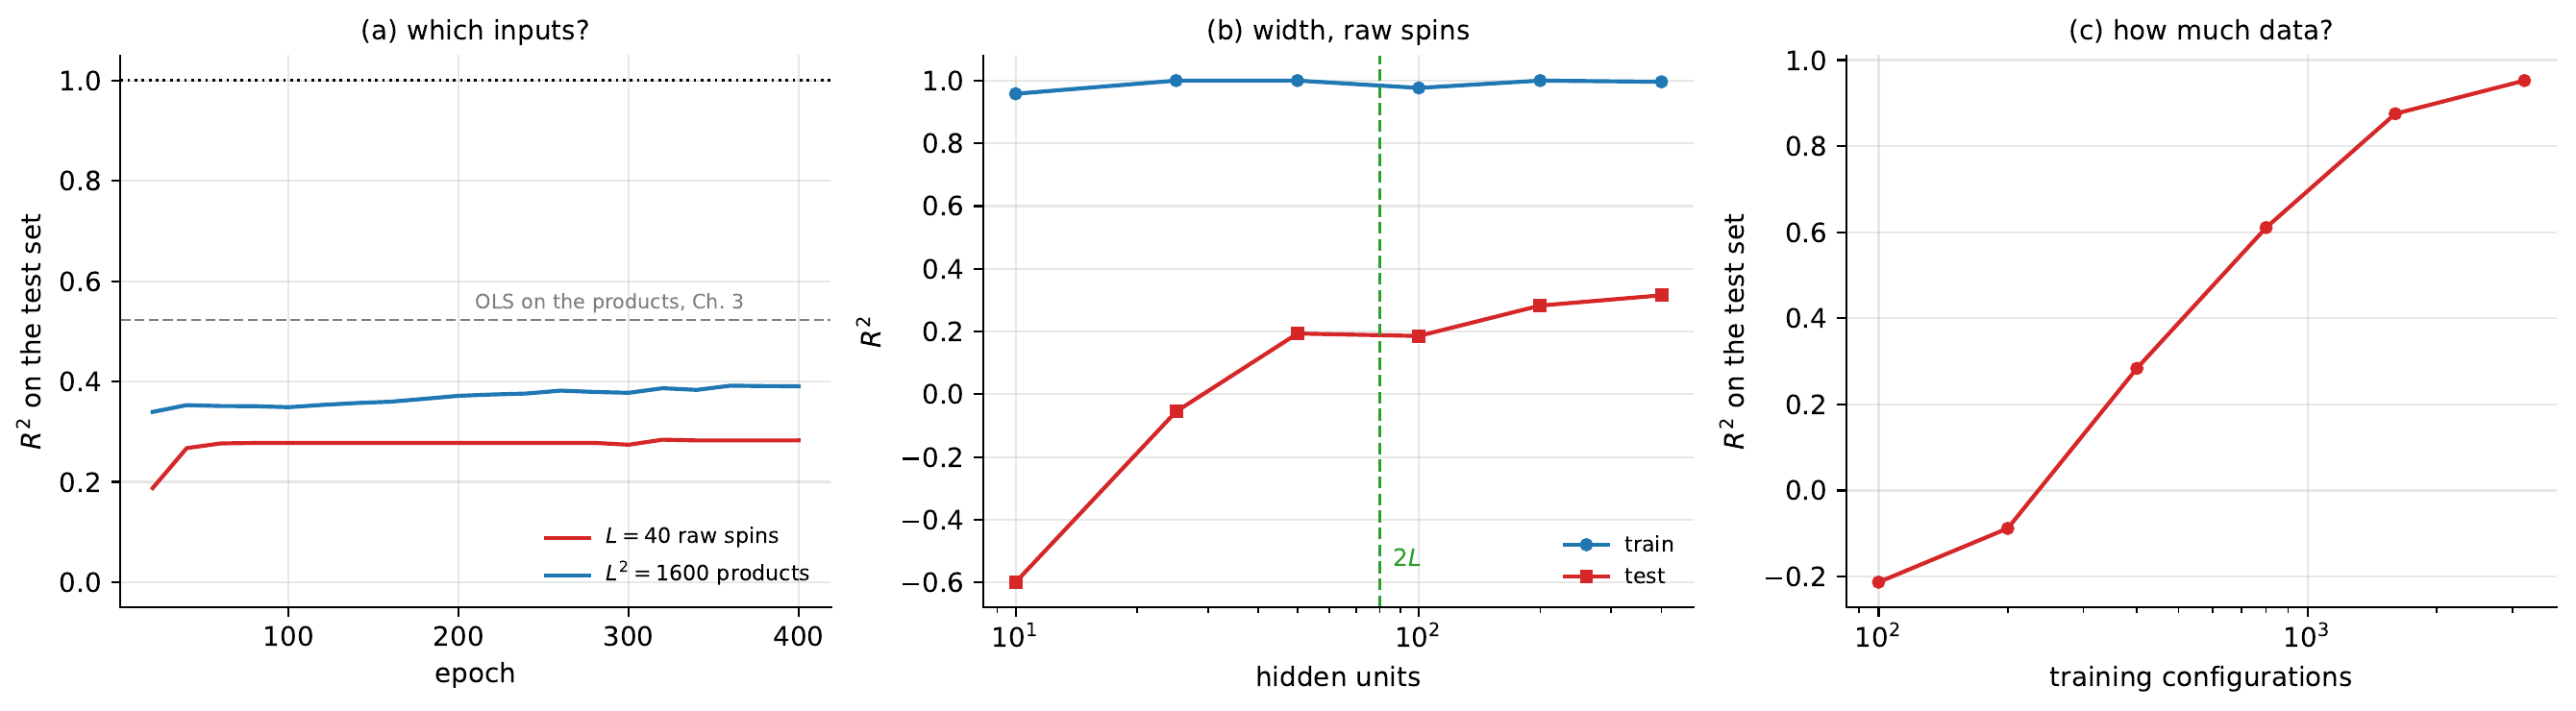
\includegraphics[width=0.98\textwidth]{BookFigures/chapter08_neural_networks/ising_network}
\caption{Learning the Ising energy with a one-hidden-layer network.  (a)
Test $R^{2}$ against epoch for the $L=40$ raw spins and for the $L^{2}=1600$
products of Section~\ref{sec:ising}, both from $400$ training configurations.
(b) Width study on the raw spins; the dashed line marks the $2L$ units that
suffice for the exact representation of
Proposition~\ref{prop:8-isingexact}.  (c) Test $R^{2}$ against the number of
training configurations: the limitation is data, not capacity.}
\label{fig:8-isingnetwork}
\end{figure}

The gap between $R^{2}=1$, which a network of $80$ units achieves with the
right weights, and $R^{2}=0.28$, which a network of $200$ units achieves after
being trained on $400$ examples, is the whole distance between approximation
theory and machine learning.  Section~\ref{sec:universal} guarantees the
former and says nothing at all about the latter.  It is worth being explicit
about why the guarantee is silent: the theorem quantifies over functions and
asserts the existence of weights, whereas training is an optimisation over
weights driven by a finite sample, and the sample is what fails here.  With
$40$ inputs there are $780$ pairwise interactions the network could believe in,
and $400$ configurations are not enough to rule out the $740$ that are absent.

%......................................................................
\subsection{Against Chapter~\ref{chap:lreg}}
\label{sec:isingcompare}

Now the comparison the section was built for.  All models below are fitted on
the same $400$ configurations and scored on the same $9600$ held-out ones.

\begin{Python}{}
   model                            R^2 on the 9600 test configurations
   OLS,   L^2 outer products              0.522863
   Ridge, L^2 outer products              0.522863
   Lasso, L^2 outer products              0.999963
   network, L^2 outer products            0.390631
   OLS,   L raw spins                    -0.112870
   network, L raw spins                   0.282703
   exact network, L raw spins             1.000000
\end{Python}

Read from the bottom up.  A network can be perfect and a linear model on the
same inputs cannot do better than the mean -- there is the case for
nonlinearity, and it is absolute.  Trained rather than constructed, the same
network reaches $0.28$, which is better than the linear model on the same
inputs by an infinite margin and worse than the Lasso on engineered features
by a wide one.  And a network \emph{given} the engineered features scores
$0.39$, below the $0.52$ of plain OLS on those features and far below the
Lasso: told that the answer is linear, the network still has to rediscover
that fact from data, and it spends its capacity on a flexibility the problem
does not need.

The ordering is uncomfortable if one expects networks to dominate, and it is
the honest result.  Its lesson is not that networks are weak.  It is that in
the regime $n=400$, $p=1600$, with a truth that is sparse in a known basis, a
penalised linear model is the right tool, and the penalty
of Section~\ref{sec:lasso} encodes knowledge -- \emph{most interactions are
absent} -- that a network trained from scratch has to buy with data.
Figure~\ref{fig:8-isingcomparison} shows the same numbers, together with the
network's score once it is given $8000$ configurations instead of $400$,
which is where the ordering starts to reverse.

\begin{figure}[htbp]
\centering
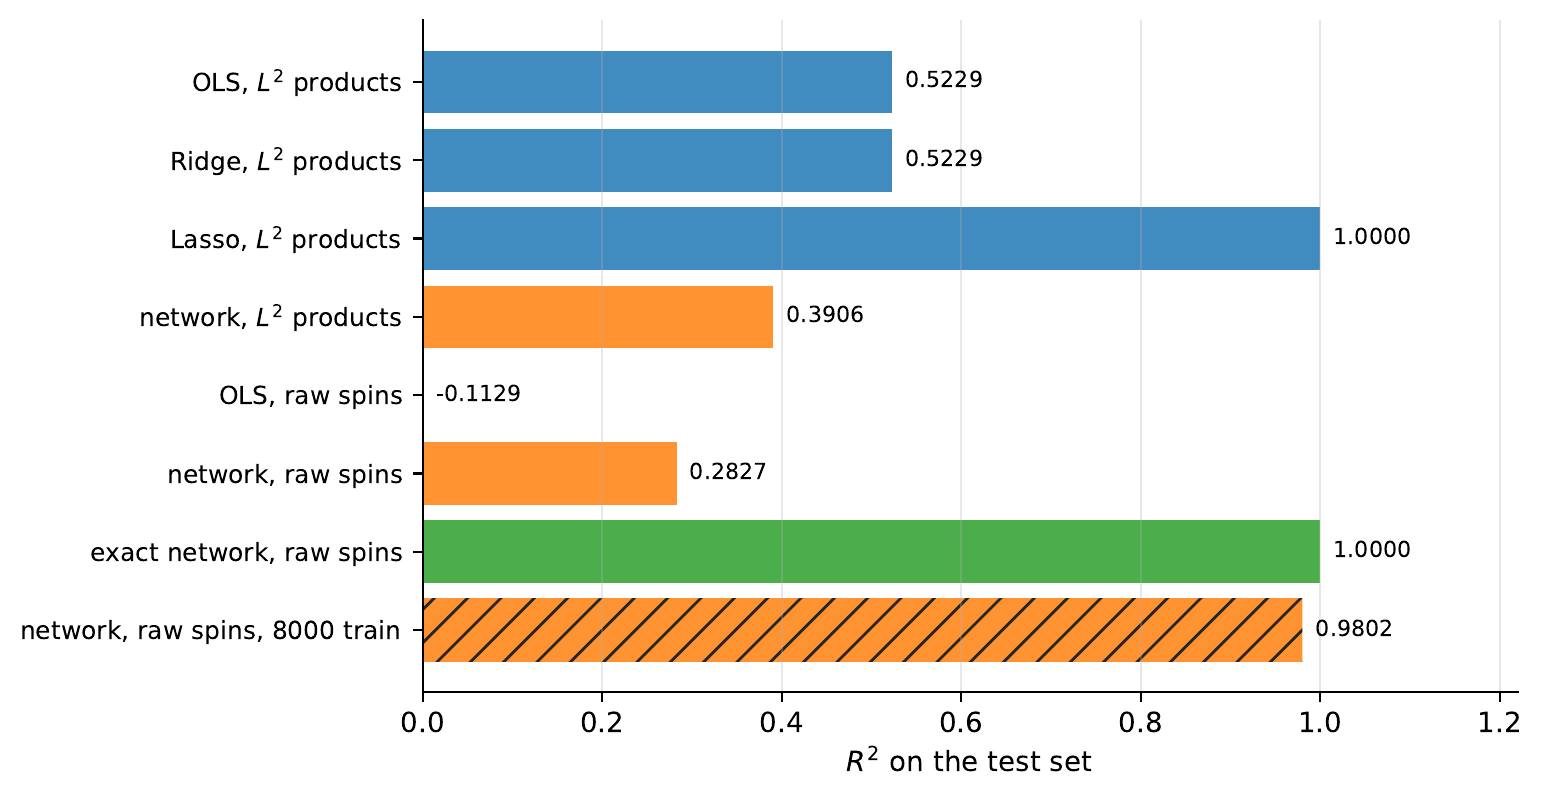
\includegraphics[width=0.85\textwidth]{BookFigures/chapter08_neural_networks/ising_comparison}
\caption{Every model of Section~\ref{sec:ising} and this section on the same
problem.  Blue: linear models.  Orange: trained networks.  Green: the exact
network of Proposition~\ref{prop:8-isingexact}.  All bars use $400$ training
configurations and the same $9600$ test configurations except the hatched one,
which uses $8000$ training configurations and a separate held-out set of
$2000$.  Negative scores are drawn as zero and labelled.}
\label{fig:8-isingcomparison}
\end{figure}

The same experiment in PyTorch, with an independent initialisation and an
independent shuffle, agrees:

\begin{Python}{}
   framework      R^2 train    R^2 test
   numpy           0.999999    0.282703
   PyTorch         0.996700    0.267799
\end{Python}

\begin{Python}{}
import torch

model = torch.nn.Sequential(
    torch.nn.Linear(L, 200), torch.nn.ReLU(), torch.nn.Linear(200, 1)
).double()
opt = torch.optim.Adam(model.parameters(), lr=3e-3)
lossf = torch.nn.MSELoss()
for ep in range(400):
    perm = torch.randperm(ntr)
    for s in range(0, ntr, 40):
        b = perm[s:s + 40]
        opt.zero_grad()
        lossf(model(Xt[b]).squeeze(-1), yt[b]).backward()
        opt.step()
\end{Python}

The two do not agree digit by digit and are not meant to.  They agree on the
conclusion, which is the only thing a cross-check can establish.

\begin{notebox}
\textbf{Machine learning connection.}  The exercise of this section --
predicting the energy of a configuration of atoms or spins from the
configuration alone -- is the basis of machine-learned interatomic potentials,
which are now a standard tool in computational chemistry and materials
science.  The economics are the same as here: a quantum-mechanical energy is
expensive, a fitted surrogate is cheap, and the surrogate is only useful if it
generalises to configurations never computed.  Two features of the successful
architectures are visible in miniature in
Proposition~\ref{prop:8-isingexact}.  They are built from local terms -- each
hidden unit in Eq.~(\ref{eq:8-isingnet}) reads two neighbouring sites, not all
forty -- so the parameter count grows with the range of the interaction rather
than the size of the system.  And they enforce the symmetries of the problem
by construction rather than learning them, which is exactly the data saving
that Section~\ref{sec:isinglearn} shows is needed: our network had to spend
thousands of configurations discovering that couplings beyond nearest
neighbours are zero, whereas a locality constraint would have supplied that
for free.  Chapter~\ref{chap:cnn} makes the same argument for images under
translation, and it is the single most useful design principle in the
subject.
\end{notebox}

%----------------------------------------------------------------------
\section{Summary and the programs}
\label{sec:ch8summary}

The chapter began with a promise made in Chapter~\ref{chap:logreg}: logistic
regression is a neural network with no hidden layer.  The XOR gate showed why
that is not enough -- a single layer computes a linear boundary, and linear
regression on XOR returns the constant $0.5$ while logistic regression achieves
exactly chance -- and a hidden layer of two units solved all three gates
perfectly.

The mathematics is a composition.  A layer computes
$\bm{z}^{l}=(\bm{W}^{l})^{T}\bm{a}^{l-1}+\bm{b}^{l}$ followed by an
element-wise non-linearity; stacking layers gives the feed-forward pass, and
the universal approximation theorem guarantees that one hidden layer suffices
to represent any continuous function -- while saying nothing about how many
units are needed or whether gradient descent will find them.

The gradient follows from the chain rule alone.  Defining the error
$\delta_j^{l}=\partial C/\partial z_j^{l}$ gives the four
equations~(\ref{eq:8-bp1})--(\ref{eq:8-bp4}): the output error starts the
recursion, Eq.~(\ref{eq:8-bp2}) pulls it backwards through the transposed
weights modulated by $f'$, and the weight and bias gradients follow
immediately.  The whole gradient costs about two forward passes regardless of
the number of parameters, which is reverse-mode automatic differentiation from
Section~\ref{sec:autodiff} specialised to a layered graph.  For the natural
pairings of output activation and loss -- linear with squared error, softmax
with cross entropy -- the output error collapses to
$\bm{\delta}^{L}=\bm{a}^{L}-\bm{y}$.

Two practical problems then had to be solved before any of this worked in
depth.  Equation~(\ref{eq:8-deltaproduct}) shows the gradient reaching layer
$l$ to be a product of $L-l$ factors, which shrinks or grows geometrically;
since $\sigma'\le\tfrac14$, a ten-layer sigmoid network attenuates the gradient
by $10^{-6}$ before it reaches the first layer.  The repairs were the ReLU
family, which does not saturate, and the variance-preserving initialisations of
Eqs.~(\ref{eq:8-xavier}) and (\ref{eq:8-he}).

The implementation of Section~\ref{sec:nncode} is those equations transcribed,
and it was verified against finite differences to between $10^{-6}$ and
$10^{-8}$ for every activation function and both output heads before being used
on anything.

The complete programs are collected in \texttt{doc/BookML/BookPrograms}:

\begin{itemize}
  \item \texttt{gates.py} -- linear regression, logistic regression and a
        neural network on the AND, OR and XOR gates of
        Table~\ref{tab:gates}.
  \item \texttt{neural\_network.py} -- the activation functions and the
        \texttt{NeuralNetwork} class of Section~\ref{sec:nncode}, with the
        gradient check.
  \item \texttt{digits.py} -- the handwritten-digit example, the comparison
        against \texttt{scikit-learn}, and the depth study used in the
        exercises.
  \item \texttt{frameworks.py} -- the same network in \texttt{scikit-learn} and
        \texttt{PyTorch}.
  \item \texttt{ising\_network.py} -- the Ising study of
        Section~\ref{sec:ising8}: the vanishing spin-energy correlation of
        Proposition~\ref{prop:8-isingsymmetry}, the exact $2L$-unit network
        of Proposition~\ref{prop:8-isingexact}, width and sample-size
        studies, the comparison against the three estimators of
        Section~\ref{sec:ising}, and a \texttt{PyTorch} cross-check.
\end{itemize}

%=============================================================================
\section{Exercises}
\label{sec:ch8exercises}
%=============================================================================

\subsection*{Warm-up exercises}
\addcontentsline{toc}{subsection}{Warm-up exercises}

\begin{enumerate}

\item \textbf{Linear layers collapse.}
  (a) Show that a network with two layers and \emph{linear} activations
      computes an affine function of its input, and identify the effective
      weight matrix and bias.
  (b) Deduce that depth is useless without a non-linearity.
  (c) Does the same argument apply if only the \emph{output} layer is linear?

\item \textbf{The XOR gate by hand.}
  Construct explicitly a network with two inputs, two hidden units with the
  step activation and one output unit that computes XOR.  Hint: let one hidden
  unit compute OR and the other NAND.  Verify your weights on all four inputs.

\item \textbf{Counting parameters.}
  For an architecture $[M_0,M_1,\dots,M_L]$, show that the number of weights is
  $\sum_l M_{l-1}M_l$ and the number of biases $\sum_l M_l$.  Evaluate both for
  $[64,50,10]$ and for $[784,300,100,10]$, and compare with the number of
  training samples in the digits and MNIST data sets respectively.

\item \textbf{Derivatives of the activations.}
  (a) Verify $\sigma'=\sigma(1-\sigma)$ and $\tanh'=1-\tanh^{2}$.
  (b) Show that $\max_z\sigma'(z)=1/4$ and $\max_z\tanh'(z)=1$.
  (c) Plot $\sigma'$, $\tanh'$, $\mathrm{ReLU}'$ and $\mathrm{ELU}'$ together
      and comment on which of them can attenuate a gradient.

\item \textbf{Deriving the four equations.}
  (a) Derive Eq.~(\ref{eq:8-deltaL}) from the squared-error cost.
  (b) Show that $\delta_j^{l}=\partial C/\partial b_j^{l}$,
      Eq.~(\ref{eq:8-bp3}).
  (c) Derive the recursion~(\ref{eq:8-bp2}) using the chain rule, being explicit
      about why the sum over $k$ appears.
  (d) Show that for a softmax output with the cross entropy the output error
      reduces to $\bm{\delta}^{L}=\bm{a}^{L}-\bm{y}$.

\item \textbf{The cost of the gradient.}
  (a) Count the multiplications in one forward pass through
      $[M_0,\dots,M_L]$.
  (b) Count them in one backward pass, and show that the two are of the same
      order.
  (c) How many forward passes would a finite-difference gradient require?
      Evaluate for $[784,300,100,10]$ and comment.

\item \textbf{Gradient check (numerical).}
  Implement the network of Section~\ref{sec:nncode} and reproduce the gradient
  check.
  (a) Confirm a relative error around $10^{-6}$ or smaller.
  (b) Deliberately introduce a bug -- omit the $f'(\bm{z}^{l})$ factor in
      Eq.~(\ref{eq:8-bp2}) -- and report what the check gives, and whether the
      network still trains.
  (c) Vary $h$ from $10^{-1}$ to $10^{-12}$ and plot the discrepancy; explain
      the shape of the curve using the round-off discussion of
      Section~\ref{sec:norms}.

\item \textbf{Vanishing gradients (numerical).}
  Train networks of depth $1,2,4,8$ hidden layers of $30$ units each on the
  digits data, once with the sigmoid and once with ReLU.
  (a) For each, record the norm of the gradient at the first and the last
      hidden layer after one epoch.
  (b) Plot the ratio against depth and compare with the bound
      $4^{-(L-1)}$ implied by Eq.~(\ref{eq:8-deltaproduct}).
  (c) Which activation permits training at depth eight?

\item \textbf{Initialisation (numerical).}
  (a) Initialise all weights to zero and explain, and then verify, what
      happens.
  (b) Compare $\mathcal{N}(0,1)$, Xavier~(\ref{eq:8-xavier}) and
      He~(\ref{eq:8-he}) initialisation on a five-layer ReLU network, plotting
      the variance of the activations against layer index after one forward
      pass.
  (c) Relate what you see to Eq.~(\ref{eq:8-varz}).

\item \textbf{Architecture and regularisation (numerical).}
  On the digits data, sweep the number of hidden units from $5$ to $200$ and
  plot training and test accuracy.
  (a) Where does overfitting begin?
  (b) Add weight decay and repeat for several $\lambda$.
  (c) Compare the best network with the random forest and the gradient-boosted
      trees of Chapter~\ref{chap:ensemble} on the same split, and with the
      logistic regression of Chapter~\ref{chap:logreg}.  Comment on accuracy,
      training time and the number of hyperparameters each required.

\end{enumerate}

%----------------------------------------------------------------------
\subsection*{Project-style exercise: building a neural network}
\addcontentsline{toc}{subsection}{Project-style exercise: neural networks}

\paragraph{Part a: forward and backward.}
Implement a fully connected network from scratch, supporting an arbitrary list
of layer sizes, a choice of hidden activation, and both output heads.  Verify
the gradient against finite differences for every activation and both heads,
and report the worst relative error as a table.  Do not proceed until this
passes.

\paragraph{Part b: the gates.}
Reproduce Section~\ref{sec:xor}: linear regression, logistic regression and
your network on AND, OR and XOR.  Then find the smallest hidden layer that
solves XOR, and plot the decision boundary your network learns.

\paragraph{Part c: regression.}
Apply your network to the Franke function of Section~\ref{sec:franke} with a
linear output layer and the squared-error cost.  Compare the test error against
the OLS, Ridge and Lasso results of Chapter~\ref{chap:lreg}, at matched numbers
of parameters where possible.  Which method wins, and does the answer depend on
the noise level?

\paragraph{Part d: classification.}
Apply it to the Wisconsin data of Section~\ref{sec:wisconsin} and to the digits
data.  Report the metrics of Section~\ref{sec:classmetrics} on a test set used
once.  Compare against logistic regression, the support vector machine of
Chapter~\ref{chap:svm} and the ensembles of Chapter~\ref{chap:ensemble}.

\paragraph{Part e: optimisers and depth.}
Replace plain gradient descent by momentum, RMSProp and Adam from
Chapter~\ref{chap:optim}, sweeping the learning rate for each, and present the
results as a table like Table~\ref{tab:optimcompare}.  Then increase the depth
and study the vanishing-gradient effect directly, comparing the sigmoid with
ReLU.

\paragraph{Part f: regularisation.}
Add weight decay, early stopping and dropout, and quantify what each is worth
on your hardest problem.  Choose all hyperparameters by cross-validation on a
validation set, and report a single number on the test set at the very end.
Discuss honestly how much of the final performance came from the architecture
and how much from the tuning.
